\documentclass[11pt]{article}
\usepackage[T1]{fontenc}
\usepackage{lmodern}
\usepackage{amsmath,amssymb,amsthm,mathtools,bm}
\usepackage[margin=1in]{geometry}
\usepackage{microtype,booktabs}
\usepackage{tikz}
\usetikzlibrary{arrows.meta,positioning,fit,matrix,calc}
\usepackage[colorlinks=true,linkcolor=blue!45!black,citecolor=blue!45!black,urlcolor=blue!45!black]{hyperref}
\let\originalthebibliography\thebibliography
\renewcommand{\thebibliography}[1]{%
  \originalthebibliography{#1}%
  \addcontentsline{toc}{section}{\refname}%
  \raggedright
}
\newtheorem{theorem}{Theorem}[section]
\newtheorem{lemma}[theorem]{Lemma}
\newtheorem{proposition}[theorem]{Proposition}
\newtheorem{corollary}[theorem]{Corollary}
\theoremstyle{definition}
\newtheorem{definition}[theorem]{Definition}
\theoremstyle{remark}
\newtheorem{remark}[theorem]{Remark}
\newtheorem{example}[theorem]{Example}
\newcommand{\R}{\mathbb R}
\newcommand{\C}{\mathbb C}
\newcommand{\Z}{\mathbb Z}
\newcommand{\N}{\mathbb N}
\newcommand{\T}{\mathbb T}
\newcommand{\E}{\mathbb E}
\renewcommand{\P}{\mathbb P}
\newcommand{\dd}{\,\mathrm d}
\newcommand{\ip}[2]{\langle #1,#2\rangle}
\newcommand{\norm}[1]{\lVert #1\rVert}
\newcommand{\abs}[1]{\lvert #1\rvert}
\DeclareMathOperator{\Law}{Law}
\DeclareMathOperator{\Ran}{Ran}
\DeclareMathOperator{\Ker}{Ker}
\DeclareMathOperator{\supp}{supp}
\DeclareMathOperator{\Span}{span}
\DeclareMathOperator{\tr}{tr}
\DeclareMathOperator{\id}{id}
\allowdisplaybreaks[2]

\title{Rokhlin's multiple-mixing problem for one transformation}
\author{OpenAI}
\date{September 23, 2026}
\hypersetup{
  pdftitle={Rokhlin's multiple-mixing problem for one transformation},
  pdfauthor={OpenAI}
}
\begin{document}
\maketitle
\vspace{-1.5\baselineskip}
\begin{abstract}
Every invertible mixing probability-preserving transformation is mixing of every finite order. Thus Rokhlin's multiple-mixing problem for a single transformation has an affirmative answer.
\end{abstract}
{\small\tableofcontents}
\section{Introduction}
\label{sec:introduction}

Let $(\Omega,\mathcal F,\mu)$ be a probability space and let $T$ be an
invertible measurable transformation with measurable inverse that preserves
$\mu$. The transformation is \emph{mixing} if
\[
 \mu(A\cap T^{-n}B)\longrightarrow\mu(A)\mu(B)
 \qquad(|n|\to\infty)
\]
for every $A,B\in\mathcal F$. For an integer $k\ge2$, it is
\emph{mixing of order $k$} if
\[
 \mu\left(\bigcap_{i=1}^k T^{-t_i}A_i\right)
 \longrightarrow\prod_{i=1}^k\mu(A_i)
\]
whenever $t_1<\cdots<t_k$ are integers and
$\min_{i<k}(t_{i+1}-t_i)\to\infty$, for every fixed choice of the
measurable sets $A_i$. Invariance allows us to take $t_1=0$.

\begin{theorem}
\label{thm:main}
Every invertible mixing probability-preserving transformation is mixing
of every finite order. More explicitly, under the assumptions above, for
every $k\ge3$ and every $A_1,\ldots,A_k\in\mathcal F$,
\[
 \mu\bigl(A_1\cap T^{-n_1}A_2\cap\cdots\cap
             T^{-(n_1+\cdots+n_{k-1})}A_k\bigr)
 \longrightarrow\prod_{i=1}^k\mu(A_i)
\]
as $\min(n_1,\ldots,n_{k-1})\to\infty$ through positive integers.
No standardness or countable-generation assumption is imposed on the
original probability space.
\end{theorem}

Corollary~\ref{cor:endomorphisms-flows} extends the conclusion to mixing
endomorphisms on arbitrary probability spaces and to mixing flows whose
Koopman operators are strongly continuous on $L^1$. These consequences
are stated and proved in Section~\ref{sec:consequences}.

Theorem~\ref{thm:main} answers Rokhlin's multiple-mixing problem
affirmatively for one transformation. Rokhlin~\cite{Rokhlin1949}
introduced higher-order mixing and proved it for ergodic surjective
continuous endomorphisms of compact commutative groups with Haar
probability. The question whether ordinary mixing alone implies the next
order is presented as Rokhlin's 1949 question in de la Rue's
account~\cite[Section~1.1]{deLaRue2006}; Ryzhikov surveys the all-orders
formulation in~\cite[Section~1]{Ryzhikov2024}. We count the order by the
number of sets, as de la Rue does: order $k$ here corresponds to
multiplicity $k-1$ in Rokhlin and Ryzhikov. Neither a group structure nor
any other special form of the transformation is assumed in our theorem.

The distinction between one time generator and several is essential.
Ledrappier's zero-entropy, mixing $\Z^2$ example is not threefold
mixing~\cite{Ledrappier1978}; de la Rue explains its three-dot relation
and why a direct one-dimensional analogue fails
\cite[Sections~1.2 and~3.4, preprint version]{deLaRue2006}. On the positive side,
Kalikow proved the twofold-to-threefold implication for rank-one
transformations~\cite{Kalikow1984}. Host obtained all orders under a
singular-spectrum hypothesis~\cite{Host1991}, and Ryzhikov obtained
all-orders conclusions for mixing finite-rank automorphisms
\cite{Ryzhikov1993}. More recently, Kanigowski and Ravotti proved
that mixing locally uniformly shearing flows are mixing of all orders
\cite[Theorem~6.8]{KanigowskiRavotti2024}.
These results require structure not present in a general mixing
transformation. For strongly mixing actions of countable abelian groups
on separable probability spaces,
Bergelson and Zelada proved that the higher-order good layouts form a
strong Ramsey-large set~\cite[Theorem~1.11]{BergelsonZelada2024}; this
does not assert convergence along every diverging-gap layout required
here.

The language of joinings, originating with Furstenberg's work on
disjointness~\cite{Furstenberg1967}, makes a failure of higher-order
mixing visible as a nonproduct limit law with independent proper
marginals. Pairwise independence alone does not force a joining to be
product. For an aperiodic finite-alphabet process, Janvresse and
de la Rue show that a pairwise-independent joining in which one
coordinate is a continuous function of the other two forces positive
entropy~\cite{JanvresseDeLaRue2008}.
For the twofold/threefold question, de la Rue records both the limit
joining and a zero-entropy reduction
\cite[Propositions~3.1 and~3.2, preprint version]{deLaRue2006}.
At arbitrary order, an antecedent Pinsker-factor reduction is described
by Ryzhikov~\cite[p.~251]{Ryzhikov1997}, who attributes it to a lemma of
Thouvenot~\cite{Thouvenot1975Pinsker}. We prove below the exact
finite-alphabet, least-failure form needed here, including the passage
from a possibly nonstandard original probability space. The new
obstacle after that reduction is to control all residual interactions
of the proper-independent limit law, not merely a selected joining.
We therefore use an ordered family of array laws and prove the later
operator and cancellation steps directly. Markov-operator methods for
joinings and intertwinings provide a related precedent
\cite{Ryzhikov1994,Ryzhikov1997}; the rectangle and exact-line
statements used here are established under our specific hypotheses.

\subsection*{The structural argument}

Suppose that $k$ is the least failing order, and put $I=\{1,\ldots,k\}$.
The reduction gives a zero-entropy finite-alphabet mixing process $X$ and
centered one-site functions $f_1,\ldots,f_k$ with product correlations
bounded below by a fixed positive constant along a sequence of diverging
layouts. A single limit joining retains this failure, but independence
of all its proper marginals does not force it to be product. For each
$n\ge1$, repeated limits at sums of $n$ layouts give a law $\rho_n$
on $X^{I^n}$, with the layout indices sent to infinity in a specified
order. The law $\rho_1$ retains the correlation witness; $\rho_2$ is
an ordered square whose proper families of last-axis planes are
independent. Higher levels allow one axis to become part of a local
state while preserving that conditional-product property. No symmetry
under permutations of array axes is assumed.

We enlarge all these laws together. A local state $y$ retains an
$X$-coordinate $x(y)$ and a parameter $u(y)$; proper last-axis planes
remain independent even after conditioning on the whole parameter array.
A conditional-expectation energy construction, using the method of
sated extensions \cite{Austin2015Sated}, makes the extension saturated:
richer data in any further admissible extension do not
improve the conditional expectation of an old test. This permits a first
axis to be included in the local state while selected states on that axis
are included in the parameter. The main conditioning argument proves that
these extensions still have the prescribed relative independence. In a
square array, saturation consequently gives exact locality of row and
column conditional laws.

The next step turns that locality into a description by orthogonal lines
of functions. At a coordinate of a joint law, consider the closed span of
the conditional expectations of functions of the other coordinates.
We call this its active space. Row and column conditional-expectation
operators in a square satisfy two rectangle identities. The identities
force fixed positive parts on the intersections of the active spaces;
their polar parts form an abelian unitary group. This yields lines spanned
by modulus-one functions that can be completed along either a row or a
column so that their product is constant. The converse inclusion requires
both incident operator identities and is proved as part of the same argument.

Here the sated-extension method is implemented in an array category
whose specified conditional product laws survive countable inverse
limits. It does not require mixing of the enlarged system. The operator step
extracts multiplicatively matched orthogonal lines from concrete kernel
identities. It uses dense-range cancellation of positive operators and
does not require their inverses to be bounded.

\subsection*{From lines to the contradiction}

The parameter geometry of the square makes the active space in each
individual fibre equal to the span of its exact lines. We enumerate these
lines measurably and regard multiplication modulo constant phases as a
countable abelian group. The row laws match these groups by isomorphisms.
A counting-measure lift of the parameter laws partitions each group into
finite blocks of constant cardinality. Time permutes the blocks, and on
an abstract copy of the group this permutation is implemented by a single
automorphism. Only the motion of whole blocks is used; a uniform rule for
the time evolution of individual labels inside a block is unnecessary.

Finally, a label orbit is either dissociated on arithmetic progressions
or polynomial on such progressions. In the first case an exponential
estimate for the label functions combines with the subexponential number
of likely words in a zero-entropy process. In the second case a Hilbert-space
averaging argument reduces polynomial degree, with ordinary mixing providing
the base case. These estimates allow an arbitrary coupling of the process
and the label functions. They show that the average absolute correlation
with each moving finite block tends to zero, contradicting a positive
quantity preserved by time.

The averages appear only in this contradiction inside a hypothetical
counterexample. The conclusion of Theorem~\ref{thm:main} remains convergence
along every diverging positive-gap layout. The proof uses one time
transformation throughout; the auxiliary array indices are not additional
time generators.

Section~\ref{sec:reduction} constructs the zero-entropy witness.
Section~\ref{sec:arrays} proves saturation and square locality.
Section~\ref{sec:operators} establishes the operator description of exact
lines. Section~\ref{sec:labels} obtains measurable labels and finite blocks.
Section~\ref{sec:cancellation} proves the one-dimensional cancellation
result, Section~\ref{sec:main-proof} assembles the contradiction, and
Section~\ref{sec:consequences} proves the endomorphism and flow consequences.

\subsection*{Conventions}

We write $\T=\{z\in\C:\abs z=1\}$ for the circle group under
multiplication. Hilbert spaces are complex, with inner products linear in
the second argument, and all spans of subspaces are closed spans. Conditional laws
and identities of factors are understood modulo null sets. After passing
to the finite-alphabet factor, all random-element spaces and subsequent
extensions are standard Borel spaces, with completion when needed.
Regular conditional laws can therefore be chosen using countable
determining classes. Assertions needed in finitely many orientations or
countably many time translates are imposed on a common conull set.
We use the standard conditional-expectation convergence theorems, the
finite-partition entropy chain rule, and the spectral theorem for compact
positive operators. Their applications below take place on the indicated
probability spaces or separable Hilbert spaces.

\section{A finite-alphabet witness of zero entropy}\label{sec:reduction}

We first place a hypothetical failure in a standard probability space and
remove its positive-entropy part.  The reduction also preserves the least
order of failure.  Throughout, the entropy of a finite partition is Shannon
entropy with natural logarithms.

\begin{proposition}[Zero-entropy witness]\label{prop:zero-entropy-witness}
Suppose an invertible mixing transformation fails to be mixing of every
order.  There then exist an integer $k\geq3$, a finite alphabet $\mathcal A$,
a shift-invariant probability measure $\mu_X$ on
$X=\mathcal A^{\Z}$, and real one-site functions $f_1,\ldots,f_k$ such that
the shift $T_X$ is mixing of every order less than $k$,
\[
 \int f_i\dd\mu_X=0,\qquad \norm{f_i}_{\infty}\leq1,
 \qquad
 \lim_{n\to\infty}\frac1nH_{\mu_X}(x_1,\ldots,x_n)=0.
\]
Moreover, there are $\delta>0$ and integer layouts
\[
 0=d_1(b)<d_2(b)<\cdots<d_k(b),\qquad
 \min_{i<k}\bigl(d_{i+1}(b)-d_i(b)\bigr)\longrightarrow\infty,
\]
for which
\begin{equation}\label{eq:witness-correlation}
 \int_X\prod_{i=1}^k f_i(T_X^{d_i(b)}x)\dd\mu_X(x)\geq\delta
 \quad\text{for every }b.
\end{equation}
\end{proposition}

\begin{proof}
Let $k$ be the least failing order and choose sets witnessing failure along
layouts whose least consecutive gap tends to infinity.  Passing to a
subsequence makes the discrepancy from the product of the means have a
fixed sign and absolute value at least some $\varepsilon>0$.  Mixing at
every smaller order holds for bounded functions, by approximation with
simple functions.

Let $\alpha$ be the finite partition generated by the witnessing sets and
put $\alpha_i=T^{-i}\alpha$.  We work inside the completed factor generated
by $(\alpha_i)_{i\in\Z}$ and define its past tail by
\[
\mathcal C=\bigcap_{m\geq1}\sigma(\alpha_i:i\leq-m).
\]
All the factor $\sigma$-fields in this proof are understood with their
probability completions.
This $\sigma$-field is invariant under $T$ and $T^{-1}$.  Write $g_i$ for
the witnessing indicators and $\bar g_i=\E[g_i\mid\mathcal C]$.  Replacing
$g_i\circ T^{d_i(b)}$ by $\bar g_i\circ T^{d_i(b)}$, successively from
$i=k$ down to $i=1$, changes the product integral by a quantity tending to
zero.  Indeed, after translating the time of the factor being replaced to
zero, all earlier factors are measurable with respect to
\[
 \mathcal F_{-g}=\sigma(\alpha_i:i\leq-g),
 \qquad g=\min_{i<k}(d_{i+1}(b)-d_i(b)),
\]
and all later, already replaced factors are $\mathcal C$-measurable.
Their product has absolute value at most one.  The error at this step is
therefore at most
\[
 \norm{\E[g_i\mid\mathcal F_{-g}]-\E[g_i\mid\mathcal C]}_1,
\]
which tends to zero by the reverse martingale theorem.  The same argument
applies to the first factor, whose remaining factors are all in the tail.
Conditional expectation preserves the means, so the tail functions still
witness failure along a subsequence.

We next verify that every finite $\mathcal C$-measurable partition $\beta$
has entropy rate zero.  For a finite partition $\gamma$, write
$\gamma_i=T^{-i}\gamma$. Stationarity and
the entropy chain rule give
\begin{equation}\label{eq:entropy-past-formula}
 h(\gamma):=\lim_{n\to\infty}\frac1nH(\gamma_1,\ldots,\gamma_n)
 =H\bigl(\gamma_0\mid\sigma(\gamma_i:i<0)\bigr).
\end{equation}
For completeness, the increments in the chain rule are
$H(\gamma_0\mid\gamma_{-j},\ldots,\gamma_{-1})$; they decrease to the
right side, since the conditional probabilities of the finitely many
atoms converge and entropy is a bounded continuous function on their
probability simplex.  Their Ces\`aro averages give the asserted limit.

For any $\epsilon>0$, there is $M$ such that
\[
 H(\beta_0\mid\alpha_{-M},\ldots,\alpha_M)<\epsilon.
\]
Consequently the chain rule and monotonicity under conditioning give
\[
 H\bigl((\alpha\vee\beta)_1,\ldots,(\alpha\vee\beta)_n\bigr)
 \leq H(\alpha_{1-M},\ldots,\alpha_{n+M})+n\epsilon.
\]
After division by $n$, this proves
$h(\alpha\vee\beta)\leq h(\alpha)+\epsilon$.  The reverse inequality
follows from refinement, and hence
$h(\alpha\vee\beta)=h(\alpha)$.

On the other hand, every translate of $\beta$ belongs to the invariant
tail $\mathcal C$ and hence to the past of $\alpha$ before each fixed
time $i$. Conditioning on $\beta_1,\ldots,\beta_n$ therefore does not
add information beyond $\sigma(\alpha_j:j<i)$ in the lower bound below:
\begin{align*}
 H(\alpha_1,\ldots,\alpha_n\mid\beta_1,\ldots,\beta_n)
 &=\sum_{i=1}^n
 H(\alpha_i\mid\alpha_1,\ldots,\alpha_{i-1},\beta_1,\ldots,\beta_n)\\
 &\geq\sum_{i=1}^n H(\alpha_i\mid\sigma(\alpha_j:j<i))
 =n h(\alpha).
\end{align*}
Combining this with
\[
 H\bigl((\alpha\vee\beta)_1,\ldots,(\alpha\vee\beta)_n\bigr)
 =H(\beta_1,\ldots,\beta_n)
  +H(\alpha_1,\ldots,\alpha_n\mid\beta_1,\ldots,\beta_n)
\]
and taking rates proves $h(\beta)=0$.

Choose, once and for all, finite-valued $\mathcal C$-measurable
approximations $h_i$ to the $\bar g_i$, with values in $[0,1]$.  They can
be made sufficiently close in $L^1$ to preserve a fixed positive
discrepancy along the selected layouts: the change in either a product
integral or the product of the means is bounded by the sum of the
$L^1$ errors.  Let $\beta$ be their common finite partition.  Coding the
$\beta$-name gives a factor on $\mathcal A^{\Z}$, with its induced measure
$\mu_X$.  This is a standard probability space, its alphabet entropy rate
is $h(\beta)=0$, and its shift inherits all mixing properties of the
original transformation.  The $h_i$ become one-site functions.

Center these functions.  Expanding their centered product, every proper
subproduct tends to the product of its means, because its ordered
sublayout still has all consecutive gaps tending to infinity and contains
fewer than $k$ times.  Thus the centered product differs by $o(1)$ from
the original discrepancy.  Each centered function has supremum norm at
most one.  A change of sign in the first function, followed by discarding
finitely many layouts, gives \eqref{eq:witness-correlation}.
\end{proof}

The all-orders Pinsker-factor antecedent is described by
Ryzhikov~\cite[p.~251]{Ryzhikov1997}, with attribution there to
Thouvenot~\cite{Thouvenot1975Pinsker}. The corresponding reduction
from failure of threefold mixing appears in de la Rue's account
\cite[Proposition~3.2, preprint version]{deLaRue2006}. We included
the proof to specify the finite-alphabet witness, the replacement order,
and the entropy conclusion on an arbitrary original probability space.

From now on we fix the system and witness supplied by
Proposition~\ref{prop:zero-entropy-witness}, and put $I=\{1,\ldots,k\}$.
The rest of the proof will contradict \eqref{eq:witness-correlation}.

\section{Ordered arrays and conditional locality}\label{sec:arrays}

The next construction retains the order in which limits are taken.  Its
basic independence is along the last axis.  Additional independence and
conditional locality will be consequences of an extension argument; they
are not symmetry assumptions on the arrays.

\subsection{The initial array laws}

We interpret $I^0$ as a singleton.  For each $n\geq0$ there is a
probability law $\rho_n$ on $X^{I^n}$ with the following properties:
\begin{enumerate}
\item $\rho_0=\mu_X$, and $\rho_n$ is invariant under simultaneous $T_X$;
\item fixing any one axis at any slot gives $\rho_{n-1}$;
\item any proper family of last-axis planes is independent under
      $\rho_n$;
\item
\begin{equation}\label{eq:array-witness}
 \int_{X^I}\prod_{i\in I}f_i(x_i)\dd\rho_1(x)\geq\delta.
\end{equation}
\end{enumerate}
Here a last-axis plane is the whole array with its last coordinate fixed;
``proper'' means containing at most $k-1$ of the $k$ planes.

To construct the laws, fix a free ultrafilter on the layout indices $b$.
For $b_1,\ldots,b_n$, start with the law of
\[
 \left(T_X^{\sum_{\ell=1}^n d_{j_\ell}(b_\ell)}x
       \right)_{(j_1,\ldots,j_n)\in I^n},\qquad x\sim\mu_X.
\]
Take the ultralimit in $b_n$ first, then $b_{n-1}$, and so on.  These
limits exist on cylinder probabilities.  They are consistent
probabilities on every finite collection of alphabet coordinates and
therefore determine a probability measure on the countable product
$X^{I^n}$.  These are also successive weak ultralimits on this compact
metrizable space.  Ultralimits of bounded scalar sequences are
linear and multiplicative.

Time invariance is immediate.  Fixing one axis adds a common time
translation to all remaining entries; invariance of $\mu_X$ removes that
translation before the limits are taken.  This proves consistency for
every axis.  To verify last-axis independence, take cylinder tests on
$s\leq k-1$ distinct last-axis planes and hold $b_1,\ldots,b_{n-1}$
fixed.  Each test is then a fixed bounded function of $x$, translated by
the corresponding $d_j(b_n)$.  Mixing of order $s$ makes their product
integral converge to the product of their integrals.  Multiplicativity
of the remaining ultralimits gives independence with plane marginal
$\rho_{n-1}$; for $s=1$ this is simply the marginal assertion and
requires no mixing hypothesis. Cylinder tests determine the asserted law. Finally,
\eqref{eq:array-witness} follows from \eqref{eq:witness-correlation}.

\subsection{The class of extensions}

All spaces in the rest of the proof are standard Borel spaces, with
their probability completions when discussing measurable functions or
$\sigma$-fields.  Conditional laws are regular conditional laws.  Their
identities are equalities almost surely, determined first on countable
generating families of tests.  This permits simultaneous choices of
versions for the countably many array levels and identities below.

At level $1$, the law $\rho_1$ still carries
\eqref{eq:array-witness}. At level $2$, view $I^2$ as a square: proper
families of its columns, the last-axis planes, are independent as
whole column arrays. We have not asserted the analogous row
independence. The higher levels will let us roll a first-axis row
into one local state and retain the same last-axis contract. To do
that we enlarge every $\rho_n$ compatibly, retaining an $X$-factor and
recording a parameter at each local state.

\begin{definition}[An array object]\label{def:array-object}
An \emph{array object} consists of standard probability systems
$(Y,m_0,T_Y)$ and $(U,\nu,T_U)$, factor maps
\[
 \kappa:Y\longrightarrow X,\qquad u:Y\longrightarrow U,
\]
and probability laws $m_n$ on $Y^{I^n}$ for $n\geq0$.  All
transformations are invertible and the factor maps commute with time.
The laws satisfy the following requirements.
\begin{enumerate}
\item Each $m_n$ is invariant under simultaneous $T_Y$ and projects
coordinatewise to $\rho_n$.  For $n\geq1$, fixing any axis at a slot
gives $m_{n-1}$, and every proper family of last-axis planes is
independent under $m_n$.
\item For $n\geq1$, conditional on the complete parameter array
$(u(y_v))_{v\in I^n}$, every proper family of last-axis planes is
independent.  The conditional law of each plane is $m_{n-1}$
conditioned only on that plane's own parameter array.
\item Under $m_0$, $\kappa(y)$ and $u(y)$ are independent; in particular,
$\kappa_*m_0=\mu_X$.
\end{enumerate}
An \emph{extension} is another such object together with a local factor
map $\theta:Y'\to Y$ preserving every array law and the map to $X$,
such that the old parameter is a factor of the new parameter.  The latter
means that $u\circ\theta=\psi\circ u'$ for a time-commuting factor
$\psi:U'\to U$.
\end{definition}

We also write $x(y)=\kappa(y)$ for the $X$-coordinate of a local state.
The initial laws give an object with $Y=X$ and a constant parameter.
For an object and $n\geq1$, let
\[
 \mathcal P_n=\sigma(u(y_v):v\in I^n),\qquad
 \mathcal O_{n,j}=\sigma(y_v:v_n\ne j),\qquad
 \mathcal G_{n,j}=\mathcal P_n\vee\mathcal O_{n,j}.
\]
Thus $\mathcal P_n$ records every parameter, $\mathcal O_{n,j}$ records
every state outside plane $j$, and $\mathcal G_{n,j}$ combines both.
Saturation will prevent an extension from revealing more about an old
test through any of these three kinds of data.

The construction uses the conditional-expectation energy and inverse-limit
method of sated extensions; see
\cite[preprint version, proof of Theorem~3.11 and Lemma~3.12]{Austin2015Sated}.
We verify directly that the defining conditional product laws of our
array category survive inverse limits.

\begin{proposition}[Saturation]\label{prop:saturation}
Every array object has an extension with the following property.  For
every $n\geq1$, every $F\in L^2(m_n)$, and each
\[
 \mathcal D\in\{\mathcal P_n\}\cup
 \{\mathcal G_{n,j},\mathcal O_{n,j}:j\in I\},
\]
no extension increases the norm of $\E[F\mid\mathcal D]$ after
pullback.  More precisely, if $\theta_n$ is the coordinatewise factor
map from any extension and $\mathcal D'$ is the corresponding data in
that extension, then
\begin{equation}\label{eq:saturation-equality}
 \E[F\circ\theta_n\mid\mathcal D']
 =\E[F\mid\mathcal D]\circ\theta_n.
\end{equation}
\end{proposition}

\begin{proof}
We first check closure under sequential inverse limits.  For a sequence
of extensions, take the local state and parameter spaces to be the
spaces of compatible paths, with their consistent probability laws.
They are standard Borel spaces.  At every array level the consistent
finite-stage laws determine a law on compatible array paths.  Time acts
coordinatewise.  Projection to $X$, consistency under fixing any axis,
and unconditional last-axis independence pass to the limit by testing
finite-stage functions.  Independence of the local $X$-state and the
limiting parameter follows in the same way.

For the conditional requirement, fix a proper family $J$ of last-axis
planes and bounded functions $F_j$ on those planes, all pulled from one
finite stage.  Let $\mathcal P_n^{(s)}$ denote the full parameter array
at stage $s$, and $\mathcal P_{n-1,j}^{(s)}$ its restriction to plane $j$.
For every sufficiently large $s$, the defining property gives
\[
 \E\left[\prod_{j\in J}F_j\,\middle|\,\mathcal P_n^{(s)}\right]
 =\prod_{j\in J}\E[F_j\mid\mathcal P_{n-1,j}^{(s)}].
\]
Increasing martingale convergence on both sides gives the same identity
for the limiting parameter fields.  The factors are uniformly bounded,
so their products converge in $L^2$.  This proves both independence
and dependence of each plane law only on its own parameters, first for
finite-stage tests and then, by density, for all bounded tests.

For a fixed test and data type, the norm of the indicated conditional
expectation is nondecreasing under extension and bounded above by the
norm of the test.  At each constructed stage, choose countable dense
families of bounded tests in every $L^2(m_n)$, and list all pairs of a
test and one of the finitely many data types at that level.  Construct
successive extensions as follows.  At round $q$, process the first $q$
listed pairs from each of the first $q$ stages already constructed.
For each pair choose an extension whose projection norm is within
$2^{-q}$ of the supremum over extensions of the current stage.
There is no requirement to attain the supremum.  Append these finitely
many extensions and continue.  Every listed pair is processed
infinitely often with error tending to zero.  Taking the sequential
inverse limit gives an object $M_\infty$ in the class.

Let $Z$ be any extension of $M_\infty$, and fix a test listed at some
finite stage.  At any sufficiently late processing step, $Z$ is also an
extension of the current stage.  Its projection norm is consequently
at most that step's supremum, which is at most the chosen next-stage
norm plus $2^{-q}$.  The next-stage norm is at most the limiting norm.
Letting $q\to\infty$ proves that $Z$ cannot increase the norm for this
test.  Finite-stage functions are dense in the inverse-limit
$L^2$ spaces, and conditional expectation is a contraction.  The same
conclusion follows for every $F\in L^2(m_n)$ of $M_\infty$.

Finally, the pullback of $\mathcal D$ is contained in $\mathcal D'$.
The Pythagorean identity for these nested orthogonal projections is
\begin{align*}
 &\norm{\E[F\circ\theta_n\mid\mathcal D']}_2^2
 -\norm{\E[F\mid\mathcal D]\circ\theta_n}_2^2\\
 &\hspace{2cm}=
 \norm{\E[F\circ\theta_n\mid\mathcal D']
       -\E[F\mid\mathcal D]\circ\theta_n}_2^2.
\end{align*}
The equality of norms therefore gives \eqref{eq:saturation-equality}.
\end{proof}

We fix a saturated object for the rest of the proof.  Its enlargement
need not be mixing.  All subsequent locality assertions will come from
\eqref{eq:saturation-equality} and the defining array laws. The equality
says that observing the extension's richer parameter or outside-plane
data reveals no more about an old $L^2$ test than the corresponding old
data did.

\subsection{Conditioning on parent planes}

We record the elementary conditioning fact that will justify the
induction.  It keeps track of which parameters determine each marginal.

\begin{lemma}[Local conditioning]\label{lem:local-conditioning}
Let $E,O_1,\ldots,O_s,B$ be standard random elements.  Suppose
$E_j=e_j(E)$ and $A_j=a_j(E_j,O_j)$ are measurable, and that
\[
 \Law((O_j)_{j=1}^s\mid E)
   =\bigotimes_{j=1}^s K_j(E_j,\cdot),\qquad
 \Law(B\mid E,O_1,\ldots,O_s)=L(E,A_1,\ldots,A_s;\cdot).
\]
If $Q_j$ is the conditional law of $O_j$ given $(E_j,A_j)$, then
\begin{equation}\label{eq:local-conditioning}
 \Law((O_j)_{j=1}^s\mid E,A_1,\ldots,A_s,B)
 =\bigotimes_{j=1}^s Q_j(E_j,A_j;\cdot).
\end{equation}
\end{lemma}

\begin{proof}
The tower property shows that $K_j(E_j,\cdot)$ is also the conditional
law of $O_j$ given $E_j$.  Let $M_j(x,\cdot)$ be its image under
$o\mapsto a_j(x,o)$.  Disintegration gives, for almost every $x$ with
respect to the law of $E_j$,
\[
 K_j(x,\dd o)\delta_{a_j(x,o)}(\dd\alpha)
 =M_j(x,\dd\alpha)Q_j(x,\alpha;\dd o).
\]
Substituting $x=e_j(E)$ preserves these almost-sure identities.  The
joint law of $(E,O,A,B)$ thus factors as
\[
 \Law(E)(\dd e)
 \left[\bigotimes_{j=1}^sM_j(e_j(e),\dd\alpha_j)\right]
 L(e,\alpha;\dd b)
 \left[\bigotimes_{j=1}^sQ_j(e_j(e),\alpha_j;\dd o_j)\right].
\]
The first three factors give the law of $(E,A,B)$, proving
\eqref{eq:local-conditioning}.
\end{proof}

\begin{lemma}[Rolling an axis into the local state]\label{lem:rolled-extension}
Let $R\subset I$ satisfy $|R|\leq k-2$, and choose $a\in I\setminus R$.
There is an extension of the saturated object whose local state is
$Y'=Y^I$, with local law $m_1$, parameter
\begin{equation}\label{eq:rolled-parameter}
 u'((y_c)_{c\in I})=((u(y_c))_{c\in I},(y_c)_{c\in R}),
\end{equation}
and factor map $(y_c)_{c\in I}\mapsto y_a$.
Its level-$n$ law is $m_{n+1}$, with the first axis treated as internal
to the local state, and its time transformation is componentwise $T_Y$.
\end{lemma}

\begin{proof}
We prove the statement by induction on $|R|$, simultaneously for all
array levels and all projection slots $a\notin R$. Saturation will be
used only for extensions already supplied by smaller parent sets.
The resulting screening identity and Lemma~\ref{lem:local-conditioning}
will then verify the conditional product law for the larger parent set.
Write an entry of
the old level $n+1$ as $y_{c,w}$, where $c\in I$ is the internal axis
and $w\in I^n$ comprises the remaining axes.  The proposed projection
retains $y_{a,w}$.  It preserves every array law by axis consistency,
preserves the $X$-state through $\kappa(y_a)$, and recovers the old
parameter from \eqref{eq:rolled-parameter}.  Time invariance,
consistency, and unconditional last-axis independence for the candidate
follow directly from the old level $n+1$.

At the local level, condition on $(u(y_c))_{c\in I}$ in $m_1$.  The set
$R\cup\{a\}$ is proper.  Its states are conditionally independent,
with the law at $a$ conditioned only on $u(y_a)$.  Since the $X$-image
of that conditional law is $\mu_X$, the selected $X$-state still has
law $\mu_X$ after conditioning further on $(y_c)_{c\in R}$.
This verifies the required independence from the enlarged parameter.
If $R=\varnothing$, the remaining conditional last-axis requirement is
exactly the old condition at level $n+1$, so the base case is proved.

Now suppose $R\ne\varnothing$ and that the lemma holds for smaller
parent sets.  Fix $n\geq1$ and a missing last-axis slot $j_0$.  In the
old law $m_{n+1}$ let
\[
 E=(u(y_{c,w}))_{c,w},\qquad
 O=(y_{c,w}:w_n\ne j_0).
\]
For $j\ne j_0$, let $O_j$ be the full plane at last slot $j$, $E_j$
its old parameter array, and $A_j$ its states at internal indices
$c\in R$.  Finally, let
\[
 B=(y_{c,w}:c\in R,\ w_n=j_0)
\]
be the parent states in the missing plane.  Conditional on $E$, the
$O_j$ are independent, with each plane law depending only on $E_j$.
We claim that
\begin{equation}\label{eq:parent-screening}
 \Law(B\mid E,O)
 \text{ depends on }O\text{ only through }(A_j)_{j\ne j_0}.
\end{equation}

Enumerate $R$ and reveal its missing-plane slices one internal index
$c$ at a time.  Let $R'$ be the set of indices already revealed.
It has smaller cardinality than $R$.  The induction hypothesis supplies
a valid extension with parent set $R'$ and projection slot $c$.
Apply saturation to a bounded test $F$ of the missing-plane slice
$(y_{c,w}:w_n=j_0)$, viewed as a function on the projected old level $n$.
For the data type $\mathcal G_{n,j_0}$, the old data are the parameters
of the row at $c$ and its states outside the missing plane; the enlarged
data are $E$, all of $O$, and the already revealed missing parent
slices. More explicitly, if $B_{R'}$ denotes those already revealed
missing slices, write $A_j^{R'}$ for the states of $O_j$ at internal
indices in $R'$.  This smaller-parent extension has
$\mathcal P'_n=\sigma(E,(A_j^{R'})_{j\ne j_0},B_{R'})$,
$\mathcal O'_{n,j_0}=\sigma(O)$, and
$\mathcal G'_{n,j_0}=\sigma(E,O,B_{R'})$. Hence
\eqref{eq:saturation-equality} says exactly that
\begin{equation}\label{eq:parent-reveal}
 \E[F\mid E,O,(y_{l,w})_{l\in R',w\in I^n}]
 =\E[F\mid (u(y_{c,w}))_{w\in I^n},
                (y_{c,w}:w_n\ne j_0)].
\end{equation}
The right side is the old $m_n$ conditional kernel at the fixed
internal index $c$.  It involves only $E$ and the part of $O$ belonging
to that same $c$, and it does not depend on previously revealed missing
states.  Multiplication of these successive kernels proves
\eqref{eq:parent-screening}.

Apply Lemma~\ref{lem:local-conditioning} to the proper family of planes
$O_j$.  Conditioning on $E$, all the $A_j$, and $B$ preserves their
independence and conditions each plane only on $(E_j,A_j)$.  These are
precisely the complete enlarged parameters and each plane's own
enlarged parameters, respectively.  The law of such a plane is the
old $m_n$, now viewed as the candidate level $n-1$; its conditional law
given $(E_j,A_j)$ is therefore exactly the one required by
Definition~\ref{def:array-object}.  We have proved the requirement for
$k-1$ planes.  Marginalization proves it for every proper family.

There are only countably many levels and finitely many choices of
parents and slots at each induction step.  Testing on countable
determining classes makes all the kernel equalities simultaneous.
The induction is complete.
\end{proof}

\subsection{The square and its grouped kernels}

Introduce the disintegrations
\begin{equation}\label{eq:local-and-row-disintegrations}
 m_0(\dd y)=\int_U\eta_u(\dd y)\nu(\dd u),\qquad
 m_1(\dd\mathbf y)=\int_{U^I}\lambda_p(\dd\mathbf y)\pi(\dd p),
\end{equation}
where $\pi$ is the law of the parameter tuple under $m_1$.
The local law $\eta_u$ is concentrated on $u(y)=u$ and satisfies
\begin{equation}\label{eq:fibre-X-marginal}
 \kappa_*\eta_u=\mu_X\quad\text{for }\nu\text{-almost every }u.
\end{equation}
Every proper coordinate marginal of $\pi$ is a product of copies of
$\nu$.  Every proper coordinate marginal of $\lambda_p$ is
$\bigotimes_j\eta_{p_j}$ on those coordinates.  These assertions follow
respectively from unconditional and conditional last-axis independence
at level one.

The measure $\nu$ is $T_U$-invariant, and $\pi$ is invariant under
$T_U^I$.  Uniqueness of disintegration and time invariance give
\begin{equation}\label{eq:fibre-time-equivariance}
 \eta_{T_Uu}=(T_Y)_*\eta_u,\qquad
 \lambda_{T_U^Ip}=(T_Y^I)_*\lambda_p.
\end{equation}
By intersecting the relevant conull sets over all integer translates,
we may use these identities, the marginal assertions, and
\eqref{eq:fibre-X-marginal} on invariant conull sets.  In particular,
time carries one fibre Hilbert space to another; it need not preserve
an individual fibre.

Write the level-two state as $(y_{a,j})_{a,j\in I}$, with $a$ the first
axis (the row index) and $j$ the last axis (the column index).  Its full
parameter array and its row and column parameter tuples are
\[
 E=(u_{a,j})_{a,j\in I},\qquad
 p_a=(u_{a,j})_{j\in I},\qquad q_j=(u_{a,j})_{a\in I}.
\]
Thus the order within either tuple is the original order on $I$.
For subsets $D,J\subset I$, let
$Y_{D,J}=(y_{a,j})_{a\in D,j\in J}$; write $Y_{a,I}$ for a single row
and $Y_{I,j}$ for a single column.

\begin{proposition}[Square locality]\label{prop:square-locality}
The following properties hold in $m_2$, and can be imposed
simultaneously on one conull set of full parameter arrays $E$.
\begin{enumerate}
\item Conditional on $E$, every proper family of columns is independent,
with column $j$ having law $\lambda_{q_j}$.  Every proper family of rows
is independent, with row $a$ having law $\lambda_{p_a}$.
\item Let $R\subset I$, $|R|\leq k-2$.  Given $E$ and the full parent
rows $Y_{R,I}$, every proper family of columns is independent, and each
column has law $\lambda_{q_j}$ conditioned on its own parent entries
$Y_{R,j}$.
\item If $a\notin R$ and $j_0\in I$, then
\begin{equation}\label{eq:single-cell-locality}
 \Law(y_{a,j_0}\mid E,Y_{R,I},Y_{I,I\setminus\{j_0\}})
 =\lambda_{p_a}(\dd y_{a,j_0}\mid Y_{a,I\setminus\{j_0\}}).
\end{equation}
\end{enumerate}
There is also the following grouped form.  Partition the rows into
three nonempty groups $P,A,B$ and the columns into three nonempty groups
$r,s,t$.  At a fixed typical $E$, each grouped row
\[
 (Y_{D,r},Y_{D,s},Y_{D,t}),\quad D\in\{P,A,B\},
\]
has a three-coordinate law with pairwise independent coordinates, and
the same holds for each grouped column.  Given $Y_{P,I}$, any two
grouped columns are independent with their own column laws conditioned
on their entries in $P$.  Finally, putting
$\Lambda_A=\bigotimes_{a\in A}\lambda_{p_a}$, we have
\begin{equation}\label{eq:grouped-cell-locality}
 \Law(Y_{A,t}\mid E,Y_{P,I},Y_{I,r\cup s})
 =\Lambda_A(\dd Y_{A,t}\mid Y_{A,r},Y_{A,s}).
\end{equation}
All these grouped assertions hold for every ordering of the three row
groups and the three column groups.
\end{proposition}

\begin{proof}
Column independence in (1) is the defining conditional independence at
level two.  To obtain rows, use the extension in
Lemma~\ref{lem:rolled-extension} with parent set $R$ and projection
slot $a\notin R$.  For a bounded test $F$ of the entire projected row,
saturation for the full parameter data $\mathcal P_1$ gives
\begin{equation}\label{eq:row-given-parents}
 \E[F(Y_{a,I})\mid E,Y_{R,I}]
 =\int F\dd\lambda_{p_a}.
\end{equation}
Reveal the members of any proper row family in turn.  The previous
members number at most $k-2$, so \eqref{eq:row-given-parents} applies
at every step.  Their joint conditional law is the product of the
indicated row laws.

Assertion (2) is the conditional last-axis requirement at level one of
the extension with parents $R$.  Its local law is $m_1$ on each column,
and its own parameter there is $(q_j,Y_{R,j})$, giving precisely the
stated marginal kernel.  For (3), use the same extension and saturation
for $\mathcal G_{1,j_0}$.  The projected old data are $p_a$ and the
other entries of row $a$, while the extension data are $E$, the parents,
and all columns except $j_0$.  This gives
\eqref{eq:single-cell-locality}.

We prove the grouped assertions without interchanging array axes.
Each row group is a proper set of rows, so its full law is the product
of its individual row laws.  Within each individual row, any proper
set of column coordinates is independent.  Consequently any two
grouped cells in that grouped row are independent.  The identical
conclusion for a grouped column follows by applying the corresponding
column assertions.  Since $|P|\leq k-2$, (2) applies to the parents
$P$.  The union of any two column groups is proper, which gives the
claimed conditional independence of grouped columns.

It remains to prove \eqref{eq:grouped-cell-locality}.  We first handle
a single missing column $j_0$.  Given $E$, $Y_{P,I}$, and all other
columns, reveal $y_{a,j_0}$ successively for $a\in A$.  At each step
the parents consist of $P$ and the previously revealed rows in $A$.
Their number is at most
\[
 |P|+|A|-1=k-|B|-1\leq k-2.
\]
All their remaining entries are already known from the observed
columns.  Equation~\eqref{eq:single-cell-locality} therefore gives
the kernel of the individual row at that step.  These kernels do not
depend on the previously revealed entries in column $j_0$, and hence
\begin{equation}\label{eq:group-single-missing}
 \Law(Y_{A,j_0}\mid E,Y_{P,I},Y_{I,I\setminus\{j_0\}})
 =\bigotimes_{a\in A}
   \lambda_{p_a}(\dd y_{a,j_0}\mid Y_{a,I\setminus\{j_0\}}).
\end{equation}

Now choose $j_0\in t$, put $J=t\setminus\{j_0\}$ and
$C=r\cup s$, and retain
$W=Y_{A,J}$ as part of the output.  The set $C\cup J$ consists of
exactly $k-1$ columns.  By (2), conditional on $E$ and $Y_{P,I}$,
those columns are independent.  In each of them, $P\cup A$ is a
proper row set.  Thus the $A$-entries, even after conditioning on its
$P$-entries, have the plain product marginal
$\bigotimes_{a\in A}\eta_{u_{a,j}}$.  It follows that
\begin{equation}\label{eq:group-intermediate-marginal}
 \Law(W\mid E,Y_{P,I},Y_{I,C})
 =\bigotimes_{a\in A,\,j\in J}\eta_{u_{a,j}}.
\end{equation}
Use \eqref{eq:group-single-missing} and then integrate away the
additional states in columns $J$, retaining $W$.  Its right side
depends on those columns only through $W$, so the resulting joint
kernel for $(W,Y_{A,j_0})$ is the measure in
\eqref{eq:group-intermediate-marginal}, followed by the product of the
individual row kernels in \eqref{eq:group-single-missing}.

Under the row-group law $\Lambda_A$, the coordinates in $C\cup J$
are also independent with exactly those marginals: the rows in $A$
are independent and each row has independent proper coordinates.
Consequently the just obtained kernel is exactly the conditional law
of $Y_{A,t}$ under $\Lambda_A$ given $Y_{A,C}$.  This proves
\eqref{eq:grouped-cell-locality}, including the case $J=\varnothing$.
Only cardinalities of the groups were used, so every ordering of the
groups is allowed.  All choices are finite; the earlier convention on
kernel versions makes the assertions simultaneous.
\end{proof}

\subsection{The geometry of the parameters}

The last property needed from the square is unconditional: it describes
how a row parameter tuple and the column parameter tuples can meet.
For $a\in I$, let
\begin{equation}\label{eq:parameter-coordinate-kernel}
 K_a(u,\dd q)=\pi(\dd q\mid q[a]=u).
\end{equation}
This is a probability kernel for $\nu$-almost every $u$, because the
$a$th coordinate marginal of $\pi$ is $\nu$.

\begin{lemma}[Parameter geometry]\label{lem:parameter-geometry}
In the level-two parameter law, for every $a\in I$ and every proper
set $J\subset I$,
\begin{equation}\label{eq:parameter-geometry}
 \Law((q_j)_{j\in J}\mid p_a)
 =\bigotimes_{j\in J}K_a(p_a[j],\dd q_j).
\end{equation}
In particular, for each $i\in I$, the diagonal row and column tuples
$p_i,q_i$ are conditionally independent, with the same law
$K_i(u,\cdot)$, given their common coordinate $u=u_{i,i}$.
\end{lemma}

\begin{proof}
It is enough to prove \eqref{eq:parameter-geometry} for
$J=I\setminus\{j_0\}$, and then take marginals.  Write
\[
 Z=Y_{a,I},\qquad O=(Y_{I,j})_{j\in J},\qquad
 S=(y_{a,j})_{j\in J}.
\]
Use the extension with no parents and projection slot $a$.
Saturation for the data $\mathcal O_{1,j_0}$ says, for every bounded
row test $F$,
\begin{equation}\label{eq:unconditional-row-screening}
 \E[F(Z)\mid O]=\E[F(Z)\mid S].
\end{equation}
Since $S$ is a function of both $Z$ and $O$, this is conditional
independence of $Z$ and $O$ given $S$.  One direct verification is to
multiply \eqref{eq:unconditional-row-screening} by a bounded function
of $O$ and condition on $S$; the resulting factorization is the
conditional-independence identity.  It also gives the reversed
screening statement $\Law(O\mid Z)=\Law(O\mid S)$.

Unconditionally the columns in $O$ are independent, each with law
$m_1$.  Conditioning on their separate shared states therefore gives
\[
 \Law(O\mid Z)
 =\bigotimes_{j\in J}m_1(\dd Y_{I,j}\mid y_{a,j}).
\]
We identify the parameter image of each factor.  In a single column,
the joint law of its parameter tuple $q$ and its state $y_a$ at slot
$a$ is
\begin{equation}\label{eq:shared-state-law}
 \pi(\dd q)\eta_{q[a]}(\dd y_a).
\end{equation}
Disintegrating $\pi$ at $q[a]$ rewrites this as
\[
 \nu(\dd u)K_a(u,\dd q)\eta_u(\dd y_a).
\]
Since $u(y_a)=u$ almost surely under $\eta_u$, the conditional law
of $q$ given the shared state $y_a$ is exactly
$K_a(u(y_a),\dd q)$.  Thus
\[
 \Law((q_j)_{j\in J}\mid Z)
 =\bigotimes_{j\in J}K_a(u(y_{a,j}),\dd q_j).
\]
The right side is a function only of $p_a$, which itself is a
function of $Z$.  Conditioning down to $p_a$ proves
\eqref{eq:parameter-geometry}.

For the last assertion, take $a=i$ and retain just $j=i$.  The tuple
$p_i$ has marginal $\pi$, and its coordinate at $i$ is $u_{i,i}$.
Given $p_i$, the law of $q_i$ is $K_i(p_i[i],\cdot)$.
Disintegrating once more over that coordinate shows that
\[
 \Law(p_i,q_i\mid u_{i,i}=u)
 =K_i(u,\dd p_i)K_i(u,\dd q_i),
\]
as required.
\end{proof}

We now have two complementary descriptions of the same square.
Proposition~\ref{prop:square-locality} gives exact conditional kernels
at a fixed full parameter array.  Lemma~\ref{lem:parameter-geometry}
controls how those parameters vary.  The first description yields the
operator structure in the next section; the second will identify which
parts of that structure persist across fibres.

\section{The operator square}
\label{sec:operators}

We now fix the parameters of a square supplied by
Proposition~\ref{prop:square-locality}.  The aim is to describe the functions
at one cell that are visible both from the rest of its row and from the rest
of its column.  We shall prove that this common subspace is spanned by
unimodular functions satisfying multiplicative relations in both directions.
The proof first treats three groups of rows and three groups of columns;
varying the groups will then recover the individual coordinates.
Operator representations of joinings have a substantial precedent in
Ryzhikov's intertwining work~\cite{Ryzhikov1994,Ryzhikov1997}; the
particular rectangle identities and exact-line conclusion below are
proved from the conditional kernels of Section~\ref{sec:arrays}.

\subsection{Active spaces and exact relations}

\begin{definition}\label{def:active-space}
Let $\lambda$ be a probability law on a finite product
$S_1\times\cdots\times S_m$ of standard spaces, with coordinate variables
$Y_1,\ldots,Y_m$ and marginals $\mu_1,\ldots,\mu_m$.
The \emph{active space} at coordinate $i$ is the closed subspace
\[
 \mathcal A_i(\lambda)
 =\overline{\Span}\bigl\{
   \E_\lambda[F(Y_j:j\ne i)\mid Y_i]:F\text{ bounded and measurable}
 \bigr\}\subseteq L^2(\mu_i).
\]
An \emph{exact tuple} is a tuple of measurable functions
$\chi_i:S_i\to\T$ for which
\begin{equation}\label{eq:exact-tuple}
 \prod_{i=1}^m\chi_i(Y_i)=c\qquad\lambda\text{-almost surely},
 \qquad c\in\T.
\end{equation}
An \emph{exact line} at coordinate $i$ is a one-dimensional subspace
$\C\chi_i$ occurring in an exact tuple.  Representatives differing by a
constant of modulus one define the same line.
\end{definition}

The active spaces contain constants and are invariant under complex
conjugation.  Their orthogonal projections therefore commute with
conjugation.  Every exact line lies in the active space: solve
\eqref{eq:exact-tuple} for its representative and condition on the chosen
coordinate.

\begin{lemma}\label{lem:exact-lines}
Suppose $m\ge3$ and every $m-1$ coordinates of $\lambda$ are independent.
Distinct exact lines at any coordinate are orthogonal.  An exact line at
one coordinate has a unique tuple of partner lines at the other coordinates.
The exact tuples of lines form an abelian group under coordinatewise
multiplication, and projection to any one coordinate is a group
isomorphism onto its group of exact lines.  Each of these groups is
countable when the marginal $L^2$ spaces are separable.  Every nonconstant
exact line has zero mean.
\end{lemma}

\begin{proof}
For an exact tuple put $a_i=\abs{\int\chi_i\dd\mu_i}$.  Solving the product
relation for $\chi_i$ and using independence of the remaining coordinates
gives
\[
 a_i=\prod_{j\ne i}a_j,\qquad 0\le a_i\le1.
\]
If some $a_i=0$, at least one other $a_j$ is zero, and the same equations
then force all $a_j$ to be zero.  Otherwise put $b_i=-\log a_i$.
The equations give $2b_i=\sum_j b_j$ for every $i$; since $m\ge3$, all
$b_i$ vanish.  Thus either all means have modulus one, in which case all
the functions are constant almost surely, or all means are zero.

The quotient of two exact tuples is again exact.  If their lines differ
at one coordinate, its quotient function is nonconstant, so all quotient
means vanish.  In particular the two representatives are orthogonal at
that coordinate.  If their lines agree at one coordinate, the quotient
there is constant, forcing constant quotients everywhere.  This proves
uniqueness of partners.  Products and conjugates preserve exact tuples;
uniqueness makes multiplication of lines well defined and makes each
coordinate projection bijective.  A family of nonzero mutually orthogonal
lines in a separable Hilbert space is countable.  Comparing any exact tuple
with the constant tuple gives the final assertion.
\end{proof}

For the rest of the section, fix a parameter square $E$ in the conull set
of Proposition~\ref{prop:square-locality}, and suppress $E$ from the
notation.  Partition the rows into three nonempty groups $P,A,B$, and the
columns into three nonempty groups $r,s,t$.  A grouped cell $Y_{i,l}$ is
the tuple of states in the corresponding rectangle.  Write $\mu_{i,l}$
for its marginal and $H_{i,l}=L^2(\mu_{i,l})$.
The square locality statement supplies the following facts, for every
ordering of the three row groups and of the three column groups:
\begin{enumerate}
\item Each grouped row and each grouped column has a three-coordinate
law whose coordinates are pairwise independent.
\item Given the whole grouped row $P$, any two grouped columns are
independent.  The conditional law of each uses only its own entry in $P$.
\item Given the whole row $P$ and all columns except $t$, the conditional
law of $Y_{A,t}$ is its own row-law kernel given $Y_{A,r},Y_{A,s}$.
\end{enumerate}
These statements concern permutations of groups within each axis; no
interchangeability of the two axes is assumed.
Let $V_{i,l}$ and $W_{i,l}$ be the active spaces for the grouped row and
grouped column laws at $(i,l)$, with projections $P^V_{i,l}$ and
$P^W_{i,l}$, respectively.

\subsection{Conditional Markov operators}

Set
\[
 z=Y_{P,r},\qquad c=Y_{P,s},\qquad d=Y_{P,t},\qquad
 x=Y_{A,r},\qquad y=Y_{B,r}.
\]
The triples $(z,c,d)$ and $(z,x,y)$ are pairwise independent.  Moreover,
$(c,d)$ and $(x,y)$ are conditionally independent given $z$: the law of
column $r$ given the whole row $P$ depends only on $z$.
It follows that each individual variable in either pair is independent
of the whole opposite pair.  For example, for bounded $f,g$,
\[
 \E[f(x)g(c,d)]
 =\E\bigl[\E[f(x)\mid z]\E[g(c,d)\mid z]\bigr]
 =\E[f(x)]\E[g(c,d)].
\]
In particular, each triple formed from one variable of a pair and the
whole opposite pair has product law.

Define four conditional Markov operators, with the arrow indicating the
direction in which functions are mapped:
\begin{equation}\label{eq:square-operators}
\begin{aligned}
 L_A(x)&:H_{A,t}\longrightarrow H_{A,s},&
 L_B(y)&:H_{B,t}\longrightarrow H_{B,s},\\
 J_s(c)&:H_{B,s}\longrightarrow H_{A,s},&
 J_t(d)&:H_{B,t}\longrightarrow H_{A,t}.
\end{aligned}
\end{equation}
For instance,
\[
 (L_A(x)h)(Y_{A,s})
 =\E[h(Y_{A,t})\mid Y_{A,r}=x,Y_{A,s}]
\]
in the grouped row law.  Pairwise independence makes the source and
target marginals independent of the conditioning value, so these are
contractions between the fixed Hilbert spaces displayed above.
Their adjoints are the reverse conditional Markov operators.  Kernels
make their matrix coefficients measurable; separability then gives
strong measurability on each vector.

Figure~\ref{fig:operator-square} fixes the four cell Hilbert spaces and
the five conditioned cells. The first identity in
Lemma~\ref{lem:rectangle} compares the two paths from the lower-right
vertex to the upper-left. The second compares the paths from the
lower-left to the upper-right, using the reverse row operators.
\begin{figure}[htbp]
  \centering
  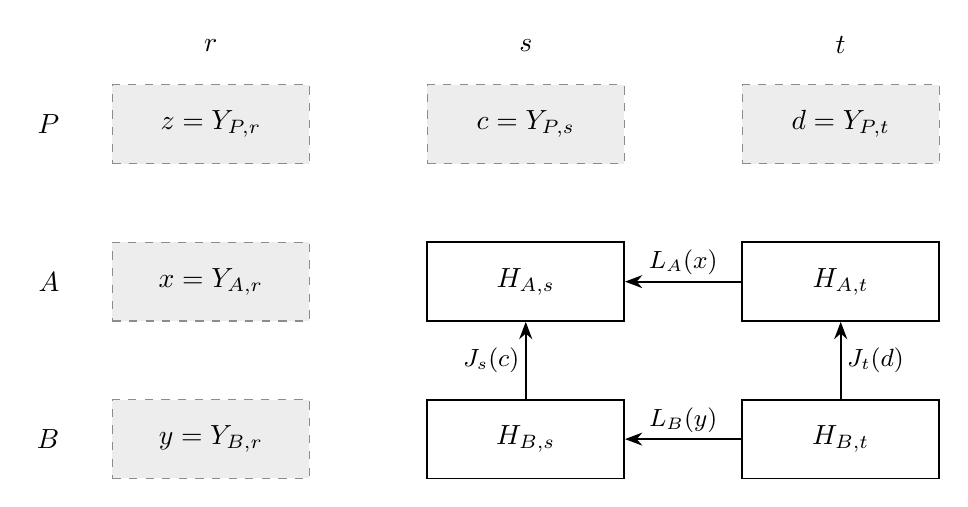
\begin{tikzpicture}[
    conditioned cell/.style={
      draw=black!45, dashed, fill=black!7,
      minimum width=25mm, minimum height=10mm,
      inner sep=3pt
    },
    operator cell/.style={
      draw=black, fill=white, line width=.6pt,
      minimum width=25mm, minimum height=10mm,
      inner sep=3pt
    },
    operator arrow/.style={-{Stealth[length=2.2mm]}, line width=.7pt},
    operator label/.style={fill=white, inner sep=2pt, font=\small}
  ]
    \node at (0,1) {$r$};
    \node at (4,1) {$s$};
    \node at (8,1) {$t$};

    \node[anchor=east] at (-1.8,0) {$P$};
    \node[anchor=east] at (-1.8,-2) {$A$};
    \node[anchor=east] at (-1.8,-4) {$B$};

    \node[conditioned cell] (Pr) at (0,0) {$z=Y_{P,r}$};
    \node[conditioned cell] (Ps) at (4,0) {$c=Y_{P,s}$};
    \node[conditioned cell] (Pt) at (8,0) {$d=Y_{P,t}$};
    \node[conditioned cell] (Ar) at (0,-2) {$x=Y_{A,r}$};
    \node[conditioned cell] (Br) at (0,-4) {$y=Y_{B,r}$};

    \node[operator cell] (As) at (4,-2) {$H_{A,s}$};
    \node[operator cell] (At) at (8,-2) {$H_{A,t}$};
    \node[operator cell] (Bs) at (4,-4) {$H_{B,s}$};
    \node[operator cell] (Bt) at (8,-4) {$H_{B,t}$};

    \draw[operator arrow] (At.west) --
      node[operator label,above] {$L_A(x)$} (As.east);
    \draw[operator arrow] (Bt.west) --
      node[operator label,above] {$L_B(y)$} (Bs.east);
    \draw[operator arrow] (Bs.north) --
      node[operator label,left] {$J_s(c)$} (As.south);
    \draw[operator arrow] (Bt.north) --
      node[operator label,right] {$J_t(d)$} (At.south);
  \end{tikzpicture}
  \caption{The grouped operator square at a fixed parameter $E$.
    The five shaded cells record the conditioned values $z,c,d,x,y$.
    Each arrow acts on functions in its source Hilbert space by
    conditional expectation in the indicated row or column law.
    Reversing an arrow represents its adjoint.}
  \label{fig:operator-square}
\end{figure}


\begin{lemma}[The rectangle identities]\label{lem:rectangle}
For the grouped square just described, almost surely in $(z,c,d,x,y)$,
\begin{equation}\label{eq:rectangle-identities}
 L_A(x)J_t(d)=J_s(c)L_B(y),\qquad
 L_A(x)^*J_s(c)=J_t(d)L_B(y)^*.
\end{equation}
The identities also hold in every ordering of the row and column groups.
\end{lemma}

\begin{proof}
Condition on $z,c,d,x,y$.  The marginal law of the two remaining entries
in column $s$ is the column law given $c$, and similarly column $t$ has
its law given $d$.  Indeed, given row $P$, each of these columns is
independent of column $r$.  Denote the corresponding two joint $L^2$
spaces by $\mathcal H_s$ and $\mathcal H_t$.
Let $Q:\mathcal H_t\to\mathcal H_s$ be the conditional Markov operator
between them under this five-cell conditioning, and let
$\iota_{A,s},\iota_{B,s},\iota_{A,t},\iota_{B,t}$ be the isometric
embeddings of the individual cell spaces into the appropriate joint
spaces.

The own-row kernel assertion gives
\[
 Q\iota_{A,t}=\iota_{A,s}L_A,\qquad
 Q\iota_{B,t}=\iota_{B,s}L_B.
\]
The same assertion with $s$ and $t$ reversed gives
\[
 Q^*\iota_{A,s}=\iota_{A,t}L_A^*,\qquad
 Q^*\iota_{B,s}=\iota_{B,t}L_B^*.
\]
Also $J_s=\iota_{A,s}^*\iota_{B,s}$ and
$J_t=\iota_{A,t}^*\iota_{B,t}$.  Consequently
\[
 L_AJ_t=\iota_{A,s}^*Q\iota_{B,t}=J_sL_B,
 \qquad
 L_A^*J_s=\iota_{A,t}^*Q^*\iota_{B,s}=J_tL_B^*.
\]
Countable dense sets of tests make these operator equalities simultaneous
on a conull set.  The grouped locality assertions hold for all the
indicated orderings, so the same proof applies to each of them.
\end{proof}

We next identify the subspaces on which the rectangle identities carry
information.  For a measurable operator family, its \emph{essential
closed range span} means the smallest closed subspace containing its
ranges for almost every parameter value.

\begin{lemma}\label{lem:active-reduction}
In every grouped cell, the projections $P^V$ and $P^W$ commute.  Every row
Markov operator intertwines the column-active projections at its source
and target; every column Markov operator intertwines the row-active
projections.  Put
\[
 D_{i,l}=V_{i,l}\cap W_{i,l},\qquad
 P^D_{i,l}=P^V_{i,l}P^W_{i,l}.
\]
Each $D_{i,l}$ is invariant under conjugation, and $P^D_{i,l}$ commutes
with conjugation.
All incident row and column operators intertwine the $P^D$ projections.
For either choice of source in a row or column, the restrictions to $D$
have essential closed range span equal to the target $D$; the same holds
for the reverse operators.
\end{lemma}

\begin{proof}
First, the essential closed range span of $L_A(x)$ is $V_{A,s}$.
Conditional expectations of product tests onto $Y_{A,s}$ have the form
\begin{equation}\label{eq:weighted-ranges}
 \int w(x)L_A(x)h\dd\mu_{A,r}(x),
\end{equation}
where $w,h$ are bounded.  Such tests span the active space by density of
product functions in the $L^2$ space of the other two coordinates.
A vector orthogonal to every integral in \eqref{eq:weighted-ranges} is
orthogonal to $L_A(x)h$ almost everywhere, by varying $w$.  A countable
dense set of $h$ then makes it orthogonal to the whole range for almost
every $x$.  The converse is immediate.  This proves the assertion, and
the same argument applies to every incident operator in either direction.
In particular each such operator has its range in its own-direction
active space and annihilates the orthogonal complement of the source
active space.

By the first rectangle identity, $J_s(c)L_B(y)$ has range in $V_{A,s}$.
The pair $(c,y)$ is independent.  Fubini and the essential range span of
$L_B$ therefore give
$J_s(c)V_{B,s}\subseteq V_{A,s}$ for almost every $c$.
The adjoint of the second identity is
$J_s(c)^*L_A(x)=L_B(y)J_t(d)^*$.
Independence of $(c,x)$ gives the reverse inclusion for the adjoint.
Together these say
\begin{equation}\label{eq:column-intertwining}
 P^V_{A,s}J_s(c)=J_s(c)P^V_{B,s}.
\end{equation}
Likewise, the first rectangle identity and independence of $(x,d)$
show that $L_A(x)W_{A,t}\subseteq W_{A,s}$; the second identity and
independence of $(x,c)$ give the adjoint assertion.  Thus
\begin{equation}\label{eq:row-intertwining}
 P^W_{A,s}L_A(x)=L_A(x)P^W_{A,t}.
\end{equation}
The same reasoning works at every edge.

Equation~\eqref{eq:column-intertwining} shows that $P^V_{A,s}$ preserves
the essential range span of $J_s$, which is $W_{A,s}$.  As an orthogonal
projection it also preserves $W_{A,s}^{\perp}$, and therefore commutes
with $P^W_{A,s}$.  This proves commutation in every cell.  Combining
\eqref{eq:row-intertwining} with the own-row active-space reduction gives
$P^D_{A,s}L_A=L_AP^D_{A,t}$, and similarly for all other edges.
Finally, projecting the essential range span $V_{A,s}$ onto $D_{A,s}$
shows that the restricted ranges of $L_A$ span $D_{A,s}$:
$P^D_{A,s}\Ran L_A=\Ran(L_AP^D_{A,t})$.
The corresponding argument handles each edge and its adjoint.
\end{proof}

We have obtained commuting projections and a rectangle of contractions
between their intersections.  The next two lemmas show that the parameter
dependence of this rectangle is carried by an abelian group of unitaries.
That description will produce exact functions at the corner cell.

\subsection{Fixed positive parts and an abelian unitary group}

Restrict the four operators in \eqref{eq:square-operators} to the $D$
spaces.  Temporarily denote them, in the same order, by $F(x)$, $G(y)$,
$K(c)$ and $N(d)$.  Their equations are
\begin{equation}\label{eq:restricted-rectangle}
 FN=KG,\qquad F^*K=NG^*.
\end{equation}
All four families and their adjoints have the essential range spans
proved in Lemma~\ref{lem:active-reduction}.

\begin{lemma}[Fixed squares]\label{lem:fixed-squares}
For the four restricted families in \eqref{eq:restricted-rectangle},
each source square and target square is independent of its parameter
almost surely, and each is injective on its $D$ space.  The four polar
parts are measurable families of unitaries between the $D$ spaces and
satisfy the first rectangle identity.
\end{lemma}

\begin{proof}
The two rectangle equations and their adjoints imply
\begin{align}
 KK^*F&=FNN^*,& K^*KG&=GN^*N,\label{eq:squares-first}\\
 F^*FN&=NG^*G,& FF^*K&=KGG^*.
 \label{eq:squares-second}
\end{align}
The parameter triples in these four equations are, respectively,
$(c,x,d)$, $(c,y,d)$, $(x,d,y)$ and $(x,c,y)$.  Each has product law by
the independence observations preceding Lemma~\ref{lem:rectangle}.

For the first equation, compare two independent values $c,c'$ using the
same $x,d$.  Fubini gives
\[
 \bigl(K(c)K(c)^*-K(c')K(c')^*\bigr)F(x)=0
\]
for almost every $(c,c',x)$.  The essential range span of $F$ is its whole
target $D$ space, so the two target squares agree.  The adjoint equation
and the essential range span of $F^*$ similarly make $NN^*$ fixed.
The second equation in \eqref{eq:squares-first} makes $K^*K$ and $N^*N$
fixed.  The two equations in \eqref{eq:squares-second}, using the range
spans of $N,K$ and their adjoints, make $F^*F,G^*G,FF^*,GG^*$ fixed.
These comparisons are operator comparisons: countable dense vector tests
first give a common conull set, after which boundedness gives equality
on every vector.

If $v$ is in the kernel of the fixed square $F^*F$, then $F(x)v=0$ for
almost every $x$.  Hence $v$ is orthogonal to the ranges of almost every
$F(x)^*$, whose essential span is the whole source $D$.  Thus $v=0$.
The same reasoning proves injectivity of all source and target squares.
Each operator consequently has zero kernel and dense range, so its polar
part has full initial and final spaces and is unitary.

To preserve the rectangle identity, put $A=|F|$ and $B=|G|$.  From
$F^*FN=NG^*G$ we obtain $A^2N=NB^2$.  Polynomial approximation to the
square-root function on $[0,1]$ gives $AN=NB$.  Write $F=U_FA$ and
$G=U_GB$.  The equation $FN=KG$ becomes
\[
 (U_FN-KU_G)B=0.
\]
The range of the injective self-adjoint $B$ is dense, so the bounded
operator in parentheses vanishes.  If $N=U_N|N|$ and $K=U_K|K|$, then
\[
 U_FN=(U_FU_N)|N|,\qquad
 KU_G=(U_KU_G)(U_G^*|K|U_G)
\]
are polar decompositions of the same operator.  Uniqueness yields
$U_FU_N=U_KU_G$.  This argument uses no inverse bound for the positive
parts.  Finally, polar parts are strongly measurable on vectors, for
example by the bounded approximations
$F(F^*F+\varepsilon\id)^{-1/2}$ as $\varepsilon\downarrow0$.
\end{proof}

Denote these polar parts by $a(x),b(y),c_0(c),d_0(d)$, respectively.  They
satisfy
\begin{equation}\label{eq:polar-rectangle}
 a(x)d_0(d)=c_0(c)b(y).
\end{equation}
The subspaces are nonzero, since constants belong to every $D$ space.

\begin{lemma}[Normalization of the polar rectangle]\label{lem:polar-group}
There are fixed unitary identifications of the four $D$ spaces with one
separable Hilbert space $\mathcal H$ such that the four polar variables
in \eqref{eq:polar-rectangle} take values in one closed abelian subgroup
$\mathcal G$ of the unitary group of $\mathcal H$.  Their common support
is $\mathcal G$.  The variables $a,b$ have a common law $\rho$, invariant
under left multiplication by every element of $\mathcal G$, and there
is a measurable $\mathcal G$-valued function $h(z)$ such that
\begin{equation}\label{eq:corner-ratio}
 a(x)b(y)^{-1}=c_0(c)d_0(d)^{-1}=h(z).
\end{equation}
The group $\mathcal G$ has a simultaneous orthonormal eigenbasis.
Monomials in its diagonal circle coordinates, evaluated at $h(z)$,
span $L^2(\sigma(h(z)))$ and are exact functions for both the row and
column three-cell laws at $(P,r)$.
\end{lemma}

\begin{proof}
Give the unitary spaces the strong operator topology.  On unitaries,
inversion and multiplication are continuous, and these spaces are
separable metrizable.  Conditional on a typical fixed value $z_0$, the
pair $(a,b)$ and the pair $(c_0,d_0)$ are independent, while each individual
marginal equals its unconditional marginal.  The continuous identity
\eqref{eq:polar-rectangle} therefore holds throughout the product of
the two conditional pair supports.
Choose one point $(a_*,b_*)$ from the first support and one point
$(c_*,d_*)$ from the second.  They satisfy $a_*d_*=c_*b_*$.  Identify the
four vertex spaces by these reference unitaries, starting at the lower
right vertex.  The two possible identifications of the upper left vertex
agree by this equation, so all four reference edge values become identity.
Use these fixed identifications from now on.

The conditional pair supports at $z_0$ now contain $(\id,\id)$.
Fixing the column pair at this point in \eqref{eq:polar-rectangle}
forces $a=b$ throughout the other pair support.  Fixing the row pair
similarly forces $c_0=d_0$.  The two row marginals therefore have a common
law $\rho$ and the two column marginals a common law $\tau$; these are
also their unconditional laws.  The supports of $\rho$ and $\tau$ both
contain identity.  Substitution of diagonal pair values into
\eqref{eq:polar-rectangle} shows that these two supports commute
elementwise.

For general $z$, conditional independence of the two pairs and their
fixed individual marginals imply
\begin{equation}\label{eq:translated-laws}
 \rho=u\rho v^{-1}
 \quad\text{for almost every actual pair }(u,v)=(c_0,d_0).
\end{equation}
Indeed, after fixing $z,c_0,d_0$, the equation says $a=c_0bd_0^{-1}$,
and $a,b$ each have law $\rho$.  Unconditionally, $c_0,d_0$ are independent,
so their pair law is $\tau\otimes\tau$.  The map
$(u,v)\mapsto u\rho v^{-1}$ is continuous for weak convergence of
probability measures: apply strong-topology continuity and dominated
convergence to each bounded continuous test.  Thus
\eqref{eq:translated-laws} holds for every $u,v\in\supp\tau$.
The symmetric argument gives $\tau=u\tau v^{-1}$ for every
$u,v\in\supp\rho$.

Taking $v=\id$ shows that each support is preserved by left translation
by elements of the other.  Because identity belongs to both, they contain
one another.  Write their common closed support as $\mathcal G$.
For $g\in\mathcal G$ we have $g\mathcal G=\mathcal G$.  This proves closure
under products, and $\id\in g\mathcal G$ supplies $g^{-1}\in\mathcal G$.
Thus $\mathcal G$ is a group.  It is abelian by the earlier commutation,
and \eqref{eq:translated-laws} gives left invariance of $\rho$.
Equation~\eqref{eq:polar-rectangle} now gives equality of the two ratios
in \eqref{eq:corner-ratio}.  Given $z$, the ratios are independent and
equal almost surely, hence have a common point-mass conditional law.
A countable determining family in the standard unitary group makes its
point measurable in $z$, giving $h$.

Choose a positive injective trace-class operator $Q$ on $\mathcal H$ and
form the trace-norm integral
\[
 Q_0=\int_{\mathcal G}UQU^*\dd\rho(U).
\]
The integrand is trace-norm continuous under strong-unitary convergence,
as follows first for finite-rank $Q$ and then by trace-norm approximation.
The integral is positive and trace-class, and left invariance of $\rho$
makes it commute with every element of $\mathcal G$.  For $v\ne0$ each
quadratic form $\ip{v}{UQU^*v}$ is positive; hence so is
$\ip{v}{Q_0v}$.  Thus $Q_0$ is injective.  Its finite-dimensional positive
eigenspaces span $\mathcal H$.  Each is invariant under the commuting
unitaries, so simultaneous diagonalization in each gives a full
orthonormal eigenbasis $(e_n)$.

Write $Ue_n=\gamma_n(U)e_n$, with $\gamma_n(U)\in\T$.
These coordinates are continuous characters.  On diagonal unitaries,
coordinatewise convergence is equivalent to strong convergence, by
approximation of any vector by its finite basis truncations.  The
coordinates therefore generate the Borel information of $\mathcal G$.
Trigonometric polynomials on every finite coordinate torus are dense in
$L^2$ of its actual probability law.  Increasing conditional expectations
onto the finite-coordinate fields then show that the functions
\[
 \gamma(h(z)),\qquad
 \gamma=\prod_{n\in J}\gamma_n^{m_n},\quad
 J\text{ finite},\quad m_n\in\Z,
\]
span $L^2(\sigma(h(z)))$.  No identification of the law of $h$ as Haar
measure is needed for this density statement.
Finally, \eqref{eq:corner-ratio} gives
\[
 \gamma(h(z))
 =\gamma(a(x))\overline{\gamma(b(y))}
 =\gamma(c_0(c))\overline{\gamma(d_0(d))}.
\]
Each factor is unimodular.  Multiplying by the conjugate factors shows
that $\gamma(h(z))$ is exact both in column $r$ and in row $P$.
\end{proof}

\subsection{Completeness of the exact functions}

Lemma~\ref{lem:polar-group} gives exact functions at the corner.  To show
that they span the entire common active subspace, we must also prove
that no other dependence remains in $D_{P,r}$.  The following projection
identity supplies this reverse inclusion.

\begin{lemma}[Projection of tensor contractions]\label{lem:contraction-completeness}
In any three-cell row of the grouped square, abbreviate the cell spaces
by $H_r,H_s,H_t$ and their common-active projections by $P_r,P_s,P_t$.
For $g\in H_s$, $h\in H_t$, set
\[
 C_r(g,h)=\E[g(Y_s)h(Y_t)\mid Y_r].
\]
Then
\begin{equation}\label{eq:contraction-projections}
 P_rC_r(g,h)=C_r(g,P_th)=C_r(P_sg,h)=C_r(P_sg,P_th).
\end{equation}
The contractions with both inputs in their $D$ spaces lie in $D_r$ and
span it.  The same assertions hold for each grouped column.
Moreover, with $h(z)$ from Lemma~\ref{lem:polar-group},
\begin{equation}\label{eq:corner-completeness}
 D_{P,r}=L^2(\sigma(h(z))).
\end{equation}
Consequently the intersection at every grouped cell is spanned by lines
exact simultaneously for its three-cell row and column laws.
\end{lemma}

\begin{proof}
Since $(Y_s,Y_t)$ has product marginal, the bilinear contraction is
well defined on $H_s\times H_t$ and satisfies
\begin{equation}\label{eq:contraction-bound}
 \norm{C_r(g,h)}_2\le\norm{g}_2\norm{h}_2.
\end{equation}
For bounded inputs let $L_{r\leftarrow t}(v)$ be the row Markov operator
from $t$ to $r$ given $Y_s=v$.  Pairwise independence gives the
vector-valued integral formula
\[
 C_r(g,h)=\int g(v)L_{r\leftarrow t}(v)h\dd\mu_s(v).
\]
Lemma~\ref{lem:active-reduction} says
$P_rL_{r\leftarrow t}(v)=L_{r\leftarrow t}(v)P_t$.
Moving the projection through the integral proves
$P_rC_r(g,h)=C_r(g,P_th)$.
Using instead the edge from $s$ to $r$ conditioned on $Y_t$ proves
$P_rC_r(g,h)=C_r(P_sg,h)$.
The bound \eqref{eq:contraction-bound} extends both identities to all
$L^2$ inputs, including unbounded projected tests.  Idempotence then gives
\[
 P_rC_r(g,h)=P_rC_r(g,P_th)=C_r(P_sg,P_th),
\]
proving \eqref{eq:contraction-projections}.  Restricted contractions are
fixed by $P_r$ and hence lie in $D_r$.  Unrestricted product contractions
span the row-active space; projecting that space onto $D_r$ proves the
restricted spanning assertion.  The column proof is identical.

Apply this result first in row $A$.  For $g\in D_{A,s}$ and
$h\in D_{A,t}$, its contraction onto $x=Y_{A,r}$ is
\[
 C_{A,r}(g,h)(x)=\ip{\overline g}{L_A(x)h}.
\]
Conjugation preserves $D_{A,s}$.  On the restricted spaces,
$L_A(x)=a(x)A_0$ for a fixed positive operator $A_0$ by
Lemma~\ref{lem:fixed-squares}.  Thus every displayed coefficient is a
function of $a(x)$ alone.  The space $L^2(\sigma(a(x)))$ is closed,
being the range of a conditional-expectation projection, so the spanning
assertion gives
\[
 D_{A,r}\subseteq L^2(\sigma(a(x))),\qquad
 D_{B,r}\subseteq L^2(\sigma(b(y))).
\]
Apply the column version of the spanning assertion in column $r$.
Given $z$, we have $a=h(z)b$ and $b$ has its fixed marginal law $\rho$.
For bounded measurable $f,g$ the contraction of $f(a)$ and $g(b)$ onto
$z$ is therefore
\[
 \int_{\mathcal G} f(h(z)u)g(u)\dd\rho(u),
\]
a function of $h(z)$.  The product marginal of $(x,y)$, the bound
\eqref{eq:contraction-bound}, and bounded approximation extend this
conclusion to the two $D$ spaces and their contraction span.  Closure
therefore yields $D_{P,r}\subseteq L^2(\sigma(h(z)))$.
In the other direction, the monomials of
Lemma~\ref{lem:polar-group} are exact for both laws, hence lie in
$D_{P,r}$, and they span $L^2(\sigma(h(z)))$.
This proves \eqref{eq:corner-completeness}.  We have used no assumption
that $D$ was already closed under multiplication.  Permuting row groups
and column groups places any grouped cell at the corner and proves the
last assertion.
\end{proof}

\subsection{From grouped cells to individual coordinates}

Return to the individual square, with row tuples $p_a$, column tuples
$q_j$, and marginal $\eta_{p_a[j]}$ at cell $(a,j)$.  Let $V_{a,j}$ be
the active space there for the full row law $\lambda_{p_a}$ and
$W_{a,j}$ the active space for the full column law $\lambda_{q_j}$.

\begin{proposition}[Common exact lines]\label{prop:common-exact-lines}
For almost every parameter square $E$, the following assertions hold
simultaneously at all individual cells.
\begin{enumerate}
\item The orthogonal projections onto $V_{a,j}$ and $W_{a,j}$ commute.
Their common range $V_{a,j}\cap W_{a,j}$ is spanned by the lines exact
for both the full $k$-coordinate row law $\lambda_{p_a}$ and the full
$k$-coordinate column law $\lambda_{q_j}$.
\item For distinct columns $s,t$, let $L^a_{s\leftarrow t}(v)$ be the
row Markov operator from cell $(a,t)$ to $(a,s)$, conditioned on the
remaining $k-2$ row entries $v$.  Then, for almost every $v$,
\[
 P^W_{a,s}L^a_{s\leftarrow t}(v)
 =L^a_{s\leftarrow t}(v)P^W_{a,t}.
\]
Column operators likewise intertwine the corresponding row-active
projections.
\item If $(\chi_j)_{j\in I}$ is an exact tuple for row $a$, with
$\prod_j\chi_j(Y_{a,j})=c$, then
\begin{equation}\label{eq:exact-partner-transport}
 L^a_{s\leftarrow t}(v)\chi_t
 =c\!\prod_{j\ne s,t}\overline{\chi_j(v_j)}\,
   \overline{\chi_s}.
\end{equation}
In particular, membership of one partner line in the column-active
space is equivalent to membership of any other partner line in its
column-active space.  The analogous assertion holds with rows and
columns exchanged.
\end{enumerate}
\end{proposition}

\begin{proof}
Isolate row $a$ and column $j$ as singleton groups, and split each of
their complements into two nonempty groups.  At the isolated cell, the
row-active and column-active spaces do not depend on the chosen splits:
the other two grouped cells still contain exactly all the other entries
of that row or column.  Lemma~\ref{lem:active-reduction} gives commutation,
and Lemma~\ref{lem:contraction-completeness} gives a spanning family of
simultaneous exact lines for the two split three-cell laws. We take this
family to contain all such lines: each is in the intersection, and
orthogonality leaves no additional line outside the spanning family.

Fix the row-group partition and vary the column-group partition.  Every
resulting family is a subset of the mutually orthogonal exact lines of
the same fixed split column law, by Lemma~\ref{lem:exact-lines}.  All have
the same closed span $V_{a,j}\cap W_{a,j}$.  Two subsets of one orthogonal
family with the same closed span must coincide: a line belonging only to
one would be orthogonal to the other span.  Now fix the initial column
grouping and vary the row grouping.  The same argument, using the fixed
split row law, shows that the initial family is exact for every split
in both directions.

For $k=3$ the grouped laws already have individual coordinates.  For
$k>3$, fix a unimodular representative $\chi_j$ of one of the lines and
consider its row completions.  For each split $S$ of $I\setminus\{j\}$,
there are unimodular functions $a_S,b_S$ and $c_S\in\T$ with
\[
 \chi_j(Y_{a,j})a_S(Y_{a,S})b_S(Y_{a,I\setminus(S\cup\{j\})})=c_S.
\]
Absorb $c_S^{-1}$ into $a_S$.  All the resulting completion functions
then equal $\overline{\chi_j(Y_{a,j})}$ under the row law, so they define
the same function $\phi$ of the other coordinates.  Those $k-1$
coordinates have product marginal.  For each singleton split, $\phi$
lies in a one-dimensional line in that coordinate tensored with the
remaining $L^2$ spaces.  The orthogonal projections to these individual
line factors commute and all fix $\phi$.  Their product has the full
one-dimensional tensor product as range, so $\phi$ is a pure product
of its unimodular individual factors, up to one scalar.  This proves
exactness for the full row law.  The column argument is the same.
Conversely, every line exact for both full laws is active for both and
belongs to their intersection.  This proves part~(1).

For part~(2), make the chosen row a singleton group, the chosen columns
$s,t$ singleton groups, and put all remaining columns in the third
group.  Split the remaining rows into two nonempty groups.  The
intertwining in Lemma~\ref{lem:active-reduction} is exactly the stated
identity for this grouping.  To obtain the column assertion, isolate
the two chosen rows instead and apply the already proved column
intertwining; there is again no interchange of axes.

Finally, solving the exact product relation for $\chi_t$ and conditioning
gives \eqref{eq:exact-partner-transport}.  Its scalar has modulus one.
The projections $P^W$ commute with conjugation.  Thus the intertwining
in part~(2) carries membership of $\C\chi_t$ in $W_{a,t}$ to membership
of $\C\chi_s$ in $W_{a,s}$.  The reverse row Markov operator gives the
converse.  The same proof applies to column partners.
\end{proof}

All constructions in this section were performed at a fixed typical
parameter square.  Kernel and operator identities can be imposed using
countable determining tests, and there are only finitely many groupings
and orientations.  The resulting conull set of parameter squares can
therefore be chosen measurable before any selection of exact lines.
The unitary reference choices and diagonal bases were needed only for
the pointwise proof: the conclusions of
Proposition~\ref{prop:common-exact-lines} concern the original conditional
laws and do not require those choices to vary measurably with $E$.
In the next section these intrinsic conclusions, together with the
parameter geometry, will identify the exact lines on individual fibres.

\section{Measurable labels and finite blocks}\label{sec:labels}

We retain the saturated array object of Section~\ref{sec:arrays}.
Its local conditional laws are $\eta_u$, its parameter-tuple law is $\pi$,
and its conditional state-tuple laws are $\lambda_p$.
Proposition~\ref{prop:common-exact-lines} describes intersections of active
spaces in a square. We must turn that intersection statement into a
description on each individual fibre. First we show that an entire
active space is spanned by exact lines. We then enumerate those lines
measurably over tuple parameters and prove that the family depends only
on the local parameter. Finally, we partition the lines into finite
sets on which time has a fixed permutation rule. One such moving set
will retain a nonzero coefficient of the original mixing witness,
providing the input for the cancellation argument in
Section~\ref{sec:cancellation}.

Write $H_u=L^2(\eta_u)$. For a tuple $p=(p_1,\ldots,p_k)$ and a slot
$i\in I$, let $\Pi_i(p)$ be the active projection in $H_{p_i}$ for
$\lambda_p$, and let $C_i(p)$ be the closed span of its exact lines.
At this point $C_i(p)$ is defined separately for each tuple; no
measurability of its line family is assumed.
We use $p_a[j]$ for the entry of row tuple $p_a$ in column $j$, so that
the row index on $p_a$ is distinguished from a coordinate of a single
tuple. Let $\vartheta$ denote the law of the complete parameter square
$E=(u_{a,j})_{a,j\in I}$.

\subsection{From intersections to entire active spaces}

The fields $H_u$ can be coordinated measurably using a countable algebra
of bounded simple functions on the standard state space and
Gram--Schmidt orthogonalization. Zero vectors are omitted, or retained
as zero padding in a fixed coordinate space $\ell^2$. These local
coordinates depend on $u$ alone. In particular, two tuple parameters
with the same entry $u$ refer to the same coordinated Hilbert space.
Conditional-expectation contractions of countably many product tests
give a measurable spanning family for each active space. Increasing
finite-dimensional projections onto these spans show that
$p\mapsto\Pi_i(p)$ is a measurable operator field.

\begin{lemma}[Active-space exactness]\label{lem:active-exact}
For $\pi$-almost every $p$ and every $i\in I$,
\begin{equation}\label{eq:active-exact}
 \Ran\Pi_i(p)=C_i(p).
\end{equation}
\end{lemma}

\begin{proof}
Fix $i$. By Lemma~\ref{lem:parameter-geometry}, the row and column
tuples meeting at cell $(i,i)$ are conditionally independent with law
\[
 \pi_i^u:=\pi(\dd p\mid p_i=u)
\]
given their common entry $u$. Proposition~\ref{prop:common-exact-lines}
therefore gives, for almost every such pair $(p,q)$,
\begin{equation}\label{eq:random-projection-intersection}
 \Pi_i(p)\Pi_i(q)=\Pi_i(q)\Pi_i(p),\qquad
 \Ran\Pi_i(p)\cap\Ran\Pi_i(q)\subseteq C_i(p).
\end{equation}

Here the almost-everywhere assertion does not presuppose a measurable
description of $C_i$. Indeed, choose a measurable conull set of
parameter squares on which the conditional kernel hypotheses of
Proposition~\ref{prop:common-exact-lines} hold on countable determining
classes. That Proposition gives its pointwise conclusion on every
square in this set. Disintegrate this set over the two tuples meeting
at $(i,i)$. On a measurable conull set of pairs the conditional measure
assigns probability one to admissible squares, and is concentrated on
the prescribed pair. Each such pair has an admissible completion.
The conclusions in \eqref{eq:random-projection-intersection} depend
only on the two tuple laws, so they hold for that pair. No measurable
choice of a completion or of an exact line is required. Disintegration
over $u$ then gives conull sections for the product law
$\pi_i^u\otimes\pi_i^u$.

For a typical $u$ define the positive contraction on $H_u$
\begin{equation}\label{eq:mean-active-projection}
 B_{i,u}=\int \Pi_i(q)\,\pi_i^u(\dd q),
 \qquad Q_{i,u}=\text{the projection onto }\Ker B_{i,u}.
\end{equation}
The weak operator integral is well defined, and its matrix entries are
measurable in $u$. Since $0\le B_{i,u}\le\id$,
$Q_{i,u}$ is the strong limit of $(\id-B_{i,u})^n$ and is measurable too.
In the fixed ambient $\ell^2$ coordinates, use the projection of each
standard basis vector $e_j$ into $H_u$ and extend the operators by zero
on $H_u^\perp$. Then
\[
 \int\norm{\Pi_i(p)Q_{i,u}e_j}^2\,\pi_i^u(\dd p)
 =\ip{Q_{i,u}e_j}{B_{i,u}Q_{i,u}e_j}=0.
\]
After a countable intersection, $\Pi_i(p)Q_{i,u}=0$ for almost every
$p$. Taking adjoints gives
\begin{equation}\label{eq:active-support}
 \Ran\Pi_i(p)\subseteq(\Ker B_{i,u})^\perp.
\end{equation}
This range containment is an operator assertion on a measurable conull
set: it is tested by $Q_{i,u}\Pi_i(p)e_j=0$ for all $j$.

Fix $p$ satisfying \eqref{eq:active-support} and having a conull
$q$-section in \eqref{eq:random-projection-intersection}.
If $v\in\Ran\Pi_i(p)$ is orthogonal to $C_i(p)$, commutation implies
that $\Pi_i(q)v$ belongs to the intersection in
\eqref{eq:random-projection-intersection}. Consequently
\[
 \norm{\Pi_i(q)v}^2=\ip{v}{\Pi_i(q)v}=0
 \quad\text{for }\pi_i^u\text{-almost every }q.
\]
Thus $\ip{v}{B_{i,u}v}=0$, and $v\in\Ker B_{i,u}$.
Equation~\eqref{eq:active-support} forces $v=0$.
The conull $q$-section used here gives whole-subspace statements, so it
works for every such $v$; a measurable selection of $v$ is unnecessary.
Every exact line is active, by its defining product relation. This
proves \eqref{eq:active-exact}. There are finitely many slots $i$.
\end{proof}

\subsection{A measurable group of lines over each local parameter}

A measurable countable family over $U$ will mean a standard measurable
space over $U$ whose fibres admit countably many measurable partial
sections enumerating them without repetition. In this description,
measurability of a fibrewise operation means measurability of its
indices in these enumerations. A line is represented by a unit vector;
for the exact lines below such a vector has modulus one almost surely.
Different scalar phases represent the same line.

\begin{proposition}[Measurable local labels]\label{prop:measurable-labels}
There is a measurable countable family of abelian groups
$u\mapsto\mathcal L(u)$, defined on a $\nu$-conull set, with the
following properties.
\begin{enumerate}
\item Each $\ell\in\mathcal L(u)$ labels a line in $H_u$ with a
measurable modulus-one representative $\chi_{u,\ell}$. The identity
label $0$ has representative $1$. Distinct labels are orthogonal,
every nonidentity representative has mean zero, and
\[
 \chi_{u,\ell}\chi_{u,\ell'}
 \in\T\chi_{u,\ell+\ell'}.
\]
\item For $\pi$-almost every $p$, the exact lines at slot $i$ of
$\lambda_p$ are precisely $\mathcal L(p_i)$, for every $i$, and they
span its active space. Unique exact matching gives measurable group
isomorphisms
\[
 \Phi_{st}(p):\mathcal L(p_s)\longrightarrow\mathcal L(p_t)
 \qquad(s,t\in I),
\]
where $\Phi_{ss}(p)=\id$.
\item Local time gives measurable group isomorphisms
\[
 \tau_u:\mathcal L(u)\longrightarrow\mathcal L(T_Uu),
 \qquad [\chi]\longmapsto[\chi\circ T_Y^{-1}].
\]
They respect exact matching. All local time assertions may be imposed
on an invariant conull set.
\item For $\vartheta$-almost every parameter square, prescribing a
label at any one cell gives a unique array of labels matched along
every row and every column.
\end{enumerate}
\end{proposition}

\begin{proof}
We first enumerate the exact lines over tuple parameters, then show
that these enumerations describe a family depending only on a local
entry. The distinction is necessary: Lemma~\ref{lem:active-exact}
alone gives no such independence from the other parameters.

\paragraph{Enumerating the tuple-dependent lines.}
Fix $i$ and another slot $j\ne i$. Let
\[
 \Delta_i(p):H_{p_i}\longrightarrow
       \bigotimes_{t\ne i}H_{p_t}
\]
be conditional expectation onto all the other coordinates under
$\lambda_p$. Their joint marginal is product, so the displayed target
is their $L^2$ space. This is a measurable contraction field. It is the
adjoint of conditional expectation in the other direction, and hence
vanishes on the inactive complement. For a unit representative of an
exact line, $\Delta_i(p)$ gives, up to a scalar phase, the unit tensor
of the conjugated matched representatives in the other slots.

Choose dense unit-ball test sections $g_n(u)$ in each $H_u$. If
$\theta_g h=g\ip{g}{h}$, set
\begin{equation}\label{eq:line-detection-operators}
 A_n(p)=\Delta_i(p)^*
   \bigl(\theta_{g_n(p_j)}\otimes\id_{t\ne i,j}\bigr)
   \Delta_i(p).
\end{equation}
All their matrix entries are measurable before any exact-line
enumeration. Pointwise, Lemma~\ref{lem:active-exact} and
Lemma~\ref{lem:exact-lines} give an orthogonal exact-line basis of the
active space. Write $w_{j,\ell}$ for the unit partner appearing at $j$
in $\Delta_i(p)\chi_\ell$. The operators in
\eqref{eq:line-detection-operators} are diagonal on this basis, with
eigenvalues
\[
 a_n(\ell)=\abs{\ip{g_n(p_j)}{w_{j,\ell}}}^2.
\]
Indeed, for two distinct labels the partners are orthogonal in every
other slot. Since $k\ge3$, at least one slot outside $i,j$ is untouched
by the insertion, and its inner product kills the off-diagonal entry.
The partners at $j$ are orthonormal, so Bessel's inequality gives
\begin{equation}\label{eq:line-operator-trace}
 \tr A_n(p)=\sum_\ell a_n(\ell)\le1.
\end{equation}
Dense tests detect each line and distinguish any two different lines:
the corresponding rank-one projections at $j$ are different.

Here is a measurable spectral construction which does not assume
that the basis just used pointwise is already enumerated measurably.
Choose independent continuously distributed weights
$w_n\in(0,2^{-n})$ and form
\[
 A(p,w)=\sum_{n\ge1}w_n A_n(p).
\]
The series converges in operator norm and is jointly measurable.
It is positive and has trace at most $\sum_n w_n$ on the conull set
where the preceding arguments apply. Trace finiteness is itself
measurable, being the finiteness of the sum of nonnegative diagonal
entries in the fixed coordinate space. Set the operator to zero on
its null exceptional set, so that the ensuing recursion always acts
on a positive compact operator.

For such an operator $A$, its norm is measurable from a countable
dense set of unit vectors. If $a=\norm A>0$, the strong limit
\[
 Q=\lim_{m\to\infty}(A/a)^m
\]
is its top-eigenvalue projection. Its matrix entries and rank are
measurable. Remove $aQ$ and repeat, taking zero projections if the
remainder is zero. Compactness ensures that this lists every distinct
positive eigenvalue and its finite-dimensional eigenspace. Thus a
repeated positive eigenvalue is detected by the measurable event that
some nonzero projection in the recursion has rank at least two.

For a fixed $p$, two distinct exact lines have different coefficient
sequences $(a_n(\ell))_n$. Conditioning on all but a weight where they
differ shows that their weighted eigenvalues coincide with probability
zero. There are only countably many lines in the separable Hilbert
space. Fubini applied to the measurable collision event therefore
chooses one deterministic sequence of weights for which the positive
spectrum is simple for almost every $p$. Every active line has a
strictly positive eigenvalue, because some test detects it and all
weights are positive. The zero eigenspace is precisely the inactive
complement; eigenvalues tending to zero add no kernel vectors. The
positive spectral projections therefore enumerate exactly the exact
lines. Zero padding of the Hilbert coordinates supplies no positive
eigenvectors and hence no extra lines.

Choose a unit vector in each one-dimensional projection by projecting
the first coordinate vector with nonzero image and normalizing.
These measurable Hilbert sections have jointly measurable function
representatives. One direct verification is to approximate a section
in each fibre within $2^{-m}$ by the first suitable member of a
countable family of rational combinations of simple sections.
The choices are measurable. The successive differences are summable
in the integrated $L^2$ norm, and hence in $L^1$, giving a measurable
almost-everywhere limit that represents the section. Each unit vector
on an exact line has modulus one, so its representative does also.
For a listed tuple of such representatives, their product $Z$ is
constant under $\lambda_p$ exactly when
\begin{equation}\label{eq:exact-tuple-test}
 \abs{\int Z\dd\lambda_p}=1.
\end{equation}
This measurable scalar test enumerates the unique matched tuples and
is unchanged by all choices of scalar phases.

\paragraph{Forcing all column memberships.}
Return to a typical parameter square. Fix a matched tuple along row
$a$, with unit representatives $v_j$ in its cells. At cell $(a,j)$ let
$Q_j$ denote the column-active projection $\Pi_a(q_j)$.
Proposition~\ref{prop:common-exact-lines} and orthogonality of distinct
row exact lines show that
\begin{equation}\label{eq:membership-indicator}
 Q_jv_j=\varepsilon_jv_j,\qquad \varepsilon_j\in\{0,1\}.
\end{equation}
Here $\varepsilon_j=1$ precisely when this row line is also an exact
line of the column law.
The row Markov operator between two cells, given the remaining cells,
intertwines their column-active projections. The exact relation maps
one chosen representative to the conjugate partner times a
modulus-one scalar depending on the remaining cells. Since the
projections commute with conjugation, this intertwining and
\eqref{eq:membership-indicator} imply
$\varepsilon_j=\varepsilon_t$ for every $j,t$.

Choose the row tuple measurably from the enumeration just obtained.
Given $p_a$, each $\varepsilon_j$ depends only on $q_j$ and this fixed
tuple. Lemma~\ref{lem:parameter-geometry} makes these indicators
pairwise conditionally independent. Their common conditional
probability $r(p_a)$ therefore satisfies $r(p_a)=r(p_a)^2$:
indeed, writing $r_j(p_a)=\E[\varepsilon_j\mid p_a]$, the almost-sure
equality of the indicators makes all $r_j$ equal, while conditional
independence gives $r_j=r_jr_t$ for $j\ne t$.
At the matched column $j=a$, however,
\[
 r(p_a)=\int\norm{\Pi_a(q)v_a}^2\,
             \pi(\dd q\mid q_a=p_a[a])
       =\ip{v_a}{B_{a,p_a[a]}v_a}>0.
\]
The strict inequality follows from \eqref{eq:active-support}, since
$v_a$ is a nonzero active vector. Thus $r(p_a)=1$.
Countably many row labels and finitely many cells make the resulting
inclusions simultaneous: every row exact line is a column exact line
at its cell, almost surely in the parameter square.

\paragraph{Descent to the local parameter.}
At $(i,i)$ two conditionally iid families of exact lines over the
shared parameter $u$ satisfy inclusion almost surely. Swapping the
two copies gives reverse inclusion, so the families agree.
To descend this agreement measurably, for each local dense test $g_n(u)$
encode a family $\mathcal S$ of orthogonal unit lines by
\begin{equation}\label{eq:line-family-encoding}
 K_n(\mathcal S)=
   \sum_{v\in\mathcal S}\abs{\ip{g_n(u)}v}^2\theta_v.
\end{equation}
The sum is independent of phases and order, has trace at most one,
and is measurable for our tuple-dependent enumeration. For every
matrix entry, the two conditional iid encodings are equal almost
surely. Their conditional squared difference is twice the conditional
variance, so that variance is zero. Each entry equals its conditional
expectation given $u$. The encodings consequently give measurable
operator fields depending only on $u$.
The family of encodings detects and distinguishes its orthogonal
lines, so the same positive-weight spectral construction recovers a
measurable family $\mathcal L_i(u)$ agreeing with the slot-$i$ exact
lines for almost every tuple with that entry.

At a nonmatched cell $(a,j)$ the already proved inclusion now reads
$\mathcal L_j(u_{a,j})\subseteq\mathcal L_a(u_{a,j})$.
The marginal of $u_{a,j}$ is $\nu$. Applying this to every ordered
pair $a,j$ yields one common family $\mathcal L(u)$ almost everywhere.
We have now removed the dependence on the other entries of a tuple:
the remaining construction can be made on the local parameter space.

By Lemma~\ref{lem:exact-lines}, multiplication of representatives
modulo scalars makes each family an abelian group. Orthogonality and
the zero-mean assertion for nonidentity labels follow from the same
Lemma. Equality of unit lines is tested by $\abs{\ip v w}=1$.
Testing the product of two representatives against the countable list
therefore makes multiplication measurable; conjugation gives the
inverse. The constant line is measurably identifiable and we choose
its representative to be $1$. Equation~\eqref{eq:exact-tuple-test}
and uniqueness give the measurable group isomorphisms $\Phi_{st}(p)$.

The equivariant versions of $\eta_u$ and $\lambda_p$ show that
composition with $T_Y^{-1}$ carries exact tuples to exact tuples.
It consequently induces $\tau_u$ and respects all matchings.
Equality tests against the measurable line lists show that this map
and its inverse are measurable. Intersecting local conull sets over
all integer translates makes the local assertions time invariant.
Tuple and square assertions are imposed separately on their own
conull sets, also intersected over integer time translates; nothing
asserts validity for every tuple over the local conull set.

\paragraph{Consistency around the square.}
Start with a matched label tuple along a row and extend every one of
its labels along its column by exact matching. Choose representatives
for the resulting labels at all cells. The product down each column
is constant under the conditional square law, as is the product
along the initial row. Dividing the product of the column relations
by that row relation shows that the product of the remaining $k-1$
row products is constant. Those rows are independent as wholes by
Proposition~\ref{prop:square-locality}. Each row product has modulus
one. The absolute mean of their product is one, so each has absolute
mean one and is itself constant. Thus every row is matched.
Starting from a single cell, its row and then all columns are uniquely
determined; the preceding argument supplies consistency along the
other rows. Countability of the label lists makes this simultaneous
for every initial label. This proves the final assertion.
\end{proof}

We now have a countable group of lines over each local parameter,
with matchings consistent across the square. It remains to find a
finite moving set of labels that retains the nonzero level-$1$
correlation.

\subsection{Counting labels and their transition operators}

We next use the parameter-square geometry to compare labels over
different local parameters. Counting measure is the appropriate
measure on each group: exact matching is a bijection, even when the
group is infinite.
Set
\[
 Z=\{(u,\ell):\ell\in\mathcal L(u)\},\qquad
 \int_Z F\dd\xi=
 \int_U\sum_{\ell\in\mathcal L(u)}F(u,\ell)\dd\nu(u)
 \quad(F\ge0).
\]
The measurable enumeration makes $\xi$ sigma-finite. The measurable
map $\tau(u,\ell)=(T_Uu,\tau_u\ell)$ preserves $\xi$, because time
preserves $\nu$ and bijects the label fibres.

\begin{lemma}[Counting lift]\label{lem:counting-lift}
There are sigma-finite measures $\widetilde\pi$ on $Z^I$ and
$\widetilde\vartheta$ on $Z^{I\times I}$, obtained by counting matched
label tuples and arrays over $\pi$ and $\vartheta$, respectively.
Every coordinate marginal is $\xi$, and each row and column marginal
of $\widetilde\vartheta$ is $\widetilde\pi$.
For $s\ne t$ the coordinate transition in $\widetilde\pi$ is the
probability kernel
\begin{equation}\label{eq:label-transition-kernel}
 K_{st}((u,\ell),A)=
 \int\mathbf1_A\bigl(p_t,\Phi_{st}(p)\ell\bigr)
                   \,\pi(\dd p\mid p_s=u).
\end{equation}
Its operator $M_{st}$ on $L^2(\xi)$ is a contraction, has adjoint
$M_{ts}$, and commutes with $V F=F\circ\tau$. For all $a\ne b$,
\begin{equation}\label{eq:label-square-identity}
 M_{st}=M_{ab}^*M_{st}M_{ab}.
\end{equation}
Given a labelled row in $\widetilde\vartheta$, any proper family of
labelled columns has the product of the column laws conditioned on
their respective shared labelled points.
\end{lemma}

\begin{proof}
For a nonnegative measurable function $F$ on $Z^I$, define
\begin{equation}\label{eq:tuple-counting-lift}
 \int F\dd\widetilde\pi
 =\int\sum_{\ell\in\mathcal L(p_s)}
 F\bigl((p_t,\Phi_{st}(p)\ell)_{t\in I}\bigr)\dd\pi(p).
\end{equation}
Unique exact matching makes this independent of the chosen source
slot $s$. Define the square measure in the same way, counting its
unique matched arrays from one chosen cell. The last assertion of
Proposition~\ref{prop:measurable-labels} makes this independent of
the chosen cell. Counting from a coordinate, row, or column gives
the claimed marginals. The preimages of the first $N$ labels of any
one coordinate have measure at most $N$ and exhaust the lifted
spaces. Thus the measures are sigma-finite.

Disintegrating \eqref{eq:tuple-counting-lift} first over $p_s=u$
gives \eqref{eq:label-transition-kernel}. For each prescribed source
label there is exactly one completion over every compatible tuple;
fixing that label introduces no weight into the parameter kernel.
This proves directly that the conditional kernels are probability
kernels even when the total lifted measure is infinite.
Similarly, given a labelled row of the square, its label has exactly
one extension over every compatible parameter square. Its conditional
parameter-square law is therefore the original law given that row's
parameter tuple. Lemma~\ref{lem:parameter-geometry} gives independent
proper columns; their labels are then determined separately by their
shared labels and their own parameter tuples. This proves the last
assertion of the Lemma.

Write $\widetilde\pi_{st}$ for the $(s,t)$ marginal.
Its two marginals are $\xi$, and its kernels in the two directions
are $K_{st}$ and $K_{ts}$. Jensen's inequality and the marginal
identities give $L^2$ contraction and $M_{st}^*=M_{ts}$.
Time equivariance of exact matching preserves both lifted measures
and gives $VM_{st}=M_{st}V$.

Finally, test the $(s,t)$ pair in row $b$ of the lifted square with
$f,g\in L^2(\xi)$. Conditional on labelled row $a$, its two column
transitions are independent applications of $M_{ab}$, since two
columns form a proper family when $k\ge3$. Hence
\begin{align*}
 \ip f{M_{st}g}
 &=\int\overline{f(z_{b,s})}\,g(z_{b,t})
                              \dd\widetilde\vartheta\\
 &=\int\overline{(M_{ab}f)(z_{a,s})}\,
                  (M_{ab}g)(z_{a,t})\dd\widetilde\vartheta\\
 &=\ip{M_{ab}f}{M_{st}M_{ab}g}
  =\ip f{M_{ab}^*M_{st}M_{ab}g}.
\end{align*}
These integrals are absolutely integrable by Cauchy--Schwarz with
the pair marginals $\xi$. Alternatively one may first use bounded
tests of finite-measure support and then pass in $L^2$.
The calculation proves \eqref{eq:label-square-identity} without
normalizing the sigma-finite measures.
\end{proof}

\subsection{Finite blocks and the time permutation}

The transition operators constrain how the countable groups can vary
with the parameter. We now extract finite pieces that have fixed sizes
and a common permutation under time. Their individual labels need not
follow a parameter-independent time rule. The construction starts with
the information transported deterministically by a transition operator.
Independence of the local parameters will make its possible values
countable; a positive $L^2$ test will make each corresponding set of
labels finite. The group matchings will then make these finite sizes
the same in almost every fibre.

\begin{lemma}[Finite label blocks]\label{lem:finite-blocks}
There are a countable index set $\mathcal B$, measurable partitions
\[
 \mathcal L(u)=\bigsqcup_{b\in\mathcal B}B_b(u)
 \quad\text{for }\nu\text{-almost every }u,
\]
and permutations $D_0,S_0$ of $\mathcal B$ with these properties.
Every $B_b(u)$ has a fixed finite positive cardinality $m_b$, independent
of $u$. For one fixed pair $s\ne t$, exact matching satisfies
\[
 \Phi_{st}(p)B_b(p_s)=B_{D_0b}(p_t)
 \quad(\pi\text{-almost every }p),
\]
and time satisfies
\[
 \tau_u B_b(u)=B_{S_0b}(T_Uu).
\]
Moreover, there are a countable abelian group $\mathcal L$, a
partition $\mathcal L=\bigsqcup_b B_b$ into sets of cardinalities $m_b$,
block-preserving group isomorphisms
$J_u:\mathcal L\to\mathcal L(u)$ for typical $u$, and an automorphism
$G$ of $\mathcal L$ such that
\begin{equation}\label{eq:abstract-block-time}
 G^r B_b=B_{S_0^{-r}b}\qquad(r\in\Z).
\end{equation}
The isomorphisms $J_u$ are only asserted to exist separately in each
fibre; they need not be chosen measurably or intertwine individual
time trajectories.
\end{lemma}

\begin{proof}
Fix $s\ne t$ and write $M=M_{st}$. Taking $(a,b)=(s,t)$ and $(t,s)$
in \eqref{eq:label-square-identity} gives
\begin{equation}\label{eq:partial-unitary-identities}
 M=M^*MM=MMM^*.
\end{equation}
Let $\mathcal H_1=\overline{\Ran M}$ and
$\mathcal H_2=\overline{\Ran M^*}$.
The first identity puts $\mathcal H_1$ in the fixed space of $M^*M$,
which lies in $\mathcal H_2$. The adjoint of the second identity puts
$\mathcal H_2$ in the fixed space of $MM^*$, which lies in
$\mathcal H_1$. They are therefore equal to a closed space
$\mathcal H$. On it $M^*M=MM^*=\id$, while
$M$ vanishes on $\mathcal H^\perp=\Ker M$.
Thus $M$ is unitary on $\mathcal H$, with inverse $M^*$ there.
For every $F\in\mathcal H$, equality in the conditional-expectation
norm gives
\begin{equation}\label{eq:deterministic-label-transition}
 F(z_t)=(MF)(z_s)
 \quad\widetilde\pi_{st}\text{-almost everywhere}.
\end{equation}
Indeed, the integral of the squared difference is
$\norm F_2^2-\norm{MF}_2^2=0$.

Choose a measurable enumeration $\ell_n(u)$ without repetition, and
set $h(u,\ell_n(u))=2^{-n}$ on its domain, starting at $n=1$.
Then $h>0$ and $\norm h_2^2\le\sum_{n\ge1}4^{-n}<\infty$.
The probability kernel sends $h$ to a strictly positive function
$v=Mh$ almost everywhere: the kernel avoids every $\xi$-null set
for almost every source point, by its marginal identity, and the
integral of a positive function under a probability law is positive.
Also $v\in\mathcal H$.

The time operator $V$ is unitary and commutes with $M$ in both
directions, so it preserves $\mathcal H$. Define the measurable
countable vector
\begin{equation}\label{eq:label-orbit-vector}
 \psi(z)=\bigl((M^nV^r v)(z)\bigr)_{(n,r)\in\Z^2}
          \in\C^{\Z^2}.
\end{equation}
Negative powers of $M$ are taken on $\mathcal H$.
All its coordinates have finite versions outside one null set, and
its $(0,0)$ coordinate is positive there. On $\C^{\Z^2}$ define
\[
 (D_0c)_{n,r}=c_{n+1,r},\qquad
 (S_0c)_{n,r}=c_{n,r+1}.
\]
These are commuting invertible coordinate reindexings.
Using \eqref{eq:deterministic-label-transition} for the countably
many coordinates gives
\begin{equation}\label{eq:psi-transports}
 \psi(z_t)=D_0\psi(z_s),\qquad
 \psi(\tau z)=S_0\psi(z)
\end{equation}
almost everywhere in the respective measures.

We claim that $\psi$ has countable essential image. Given a source
point $z=(u,\ell)$, the parameter of its $K_{st}$ target has law
$\nu$, since $p_s,p_t$ are independent under $\pi$ and fixing a
source label does not tilt that law. Consider the occurrence relation
\[
 R(z,u')\quad\Longleftrightarrow\quad
 D_0\psi(z)=\psi(u',\ell_n(u'))
 \text{ for some defined }\ell_n(u').
\]
It is measurable: existence is a countable union and equality of
vectors is a countable conjunction of coordinate equalities.
The first identity in \eqref{eq:psi-transports} implies
$\nu\{u':R(z,u')\}=1$ for $\xi$-almost every $z$.
Tonelli's theorem for the sigma-finite product $\xi\otimes\nu$
selects one $u'$ for which $R(z,u')$ holds for $\xi$-almost every
$z$. That target fibre has only countably many $\psi$-values.
Invertibility of $D_0$ proves the claim.

Let $\mathcal B$ be the positive-mass values in this countable
essential image. For $b\in\mathcal B$ put
\[
 E_b=\{z:\psi(z)=b\},\qquad
 B_b(u)=\{\ell:(u,\ell)\in E_b\}.
\]
Every $b$ has positive $(0,0)$ coordinate $b_{0,0}$, and
\begin{equation}\label{eq:finite-level-mass}
 0<\xi(E_b)\le \frac{\norm v_2^2}{|b_{0,0}|^2}<\infty.
\end{equation}
Equal marginals in the first identity of \eqref{eq:psi-transports}
and time invariance in the second show that $D_0$ and $S_0$ permute
$\mathcal B$, preserving each level's mass along their orbits.
After discarding a $\nu$-null set, all labels in every remaining
fibre belong to these levels, and each $B_b(u)$ is finite.
Countability of $\mathcal B$ makes these assertions simultaneous.

Counting the labels in \eqref{eq:psi-transports} shows that, for
$\pi$-almost every $p$, its matching isomorphism $\Phi_{st}(p)$
carries every block $b$ onto block $D_0b$.
Because each fibre's label list and $\mathcal B$ are countable,
intersecting the corresponding conull sets upgrades the transported
label identity to every label in every block for such a tuple.
Disintegrate the measurable conull set of such tuples over
$(p_s,p_t)$. Since its marginal is $\nu\otimes\nu$, there is a
measurable conull set of pairs $(u,w)$ admitting a tuple with this
property. Fubini chooses a common source $u_*$ for which almost every
target is in this set. For each such target $u$, choose one resulting
group isomorphism
$I_u:\mathcal L(u_*)\to\mathcal L(u)$.
Each $I_u$ takes block $b$ to block $D_0b$ simultaneously for every
$b$. The choices are used only pointwise.

Fix one typical target $u_0$, set $\mathcal L=\mathcal L(u_0)$,
and define $J_u=I_uI_{u_0}^{-1}$. These group isomorphisms preserve
every block index. Thus all $|B_b(u)|$ are constant almost everywhere.
Equation~\eqref{eq:finite-level-mass} makes each constant finite,
and its positive left side makes it nonzero. Let $B_b=B_b(u_0)$
and $m_b=|B_b|$.

The second identity of \eqref{eq:psi-transports} gives the asserted
time permutation of blocks. Restrict the local parameter set to
the intersection of all integer translates of the conull sets just
used and of the time-equivariance set. Choose $u$ in this invariant
conull set. The automorphism
\[
 A=J_{T_Uu}^{-1}\tau_uJ_u
\]
of $\mathcal L$ maps every $B_b$ to $B_{S_0b}$.
Take $G=A^{-1}$. Iteration gives
\eqref{eq:abstract-block-time}. This last step fixes one automorphism
realizing the permutation of blocks; it makes no assertion about
the maps inside a block at other parameters or later times.
\end{proof}

\subsection{A finite block carrying the witness}

All structural objects needed for the final argument are now
available. The next Proposition records the precise connection to
the nonzero correlation retained from the original process. Its
measurable quantities are sums over finite blocks, so the abstract
identifications in Lemma~\ref{lem:finite-blocks} will cause no
measurability issue.

\begin{proposition}[A block carrying the witness]\label{prop:block-witness}
Let the saturated array object lie over the zero-entropy finite-alphabet
mixing process $(X,\mu_X,T_X)$ supplied by
Proposition~\ref{prop:zero-entropy-witness}, with its centered
finite-valued one-site functions $f_1,\ldots,f_k$ and nonzero
level-$1$ product integral. There exist a function
$f\in\{f_1,\ldots,f_k\}$, a countable abelian group $\mathcal L$,
an automorphism $G$ of $\mathcal L$, a finite nonempty set
$B\subset\mathcal L$, and a number $c>0$ with the following properties.

For $\nu$-almost every $u$, the probability space $(Y,\eta_u)$
has factor map $x:Y\to X$ with $x_*\eta_u=\mu_X$, and admits
representatives $(\chi_\ell^u)_{\ell\in\mathcal L}$ such that
\begin{gather}
 \chi_0^u=1,\qquad |\chi_\ell^u|=1,\qquad
 \chi_\ell^u\chi_{\ell'}^u\in\T\chi_{\ell+\ell'}^u,
 \label{eq:block-character-laws}\\
 \int\chi_\ell^u\dd\eta_u=0\quad(\ell\ne0),\qquad
 \ip{\chi_\ell^u}{\chi_{\ell'}^u}_{L^2(\eta_u)}
       =\mathbf1_{\{\ell=\ell'\}}.
 \nonumber
\end{gather}
For every $r\ge0$ the function
\begin{equation}\label{eq:block-witness-sum}
 s_r(u)=\sum_{\ell\in B}
 \left|\int f(T_X^r x(y))\,
               \overline{\chi_{G^r\ell}^u(y)}\dd\eta_u(y)\right|
\end{equation}
has a measurable version and satisfies
\begin{equation}\label{eq:block-witness-integral}
 0\le s_r(u)\le |B|\norm f_\infty,
 \qquad \int_U s_r(u)\dd\nu(u)=c>0.
\end{equation}
The group identifications used to choose the representatives in
\eqref{eq:block-character-laws} need not be measurable in $u$.
Their finite sums in \eqref{eq:block-witness-sum} are intrinsic sums
over the measurable moving blocks. In particular, no time invariance
of an individual $\eta_u$ is asserted or required.
\end{proposition}

\begin{proof}
Condition the nonzero product integral at level $1$ on $p$.
For any chosen slot $i$, the conditional expectation of the product
of the other bounded inputs onto that slot belongs to its active
space. If $f_i(x)$ were orthogonal to that space for almost every
$p$, the product integral would vanish. In using complex inner
products here one can conjugate the other product; the active
space is conjugation invariant.
Lemma~\ref{lem:active-exact} and
Proposition~\ref{prop:measurable-labels} therefore give a choice
$f=f_i$ with a nonzero coefficient on some local label on a set of
positive $\nu$-measure. The identity-label coefficient is zero:
\[
 \int f(x(y))\dd\eta_u(y)=\int f\dd\mu_X=0.
\]
Thus nonidentity labels supply the nonzero coefficient.

For a block $b\in\mathcal B$ define the measurable function
\[
 c_b(u)=\sum_{\ell\in B_b(u)}
 \left|\int f(x(y))\overline{\chi_{u,\ell}(y)}\dd\eta_u(y)\right|.
\]
The countably many blocks cover all labels, so some fixed block $b$
has $\int c_b\dd\nu>0$. Its cardinality $m_b$ is fixed and finite,
and hence $c_b\le m_b\norm f_\infty$.
Set $B=B_b\subset\mathcal L$ using
Lemma~\ref{lem:finite-blocks}, and $c=\int c_b\dd\nu$.

For each typical $u$ choose the block-preserving identification $J_u$
from that Lemma and put
$\chi_\ell^u=\chi_{u,J_u\ell}$.
Proposition~\ref{prop:measurable-labels} gives
\eqref{eq:block-character-laws}.
By \eqref{eq:abstract-block-time}, the sum in
\eqref{eq:block-witness-sum} equals the intrinsic measurable sum
\begin{equation}\label{eq:intrinsic-moving-block-sum}
 \sum_{\ell'\in B_{S_0^{-r}b}(u)}
 \left|\int f(T_X^r x(y))
                  \overline{\chi_{u,\ell'}(y)}\dd\eta_u(y)\right|.
\end{equation}
Only the set of lines is relevant; changing representative phases
or permuting labels inside this set changes no summand magnitude.
This proves measurability without a measurable choice of $J_u$.

The conditional laws are equivariant:
$(T_Y^r)_*\eta_u=\eta_{T_U^r u}$.
Time carries $B_{S_0^{-r}b}(u)$ bijectively onto
$B_b(T_U^r u)$, taking representatives to representatives up to
scalar phase. The change of variables $y'=T_Y^r y$ in
\eqref{eq:intrinsic-moving-block-sum} consequently gives
\begin{equation}\label{eq:witness-block-transport}
 s_r(u)=c_b(T_U^r u).
\end{equation}
Invariance of $\nu$ proves its integral is $c$ for every $r$.
Finally, $G^r$ bijects $B$ onto $B_{S_0^{-r}b}$, so every moving
block has the same cardinality $|B|=m_b$. Each coefficient is at
most $\norm f_\infty$. This proves the bound in
\eqref{eq:block-witness-integral} and completes the Proposition.
\end{proof}

Proposition~\ref{prop:block-witness} leaves a problem on a single
probability fibre: show that the absolute coefficients along each
orbit $G^r\ell$ have Ces\`aro mean zero. The uniform finite-block
bound will then allow integration over $u$. The next section proves
this cancellation using only the mixing zero-entropy $X$ marginal
and the group relations \eqref{eq:block-character-laws}.

\section{Cancellation in one time dimension}
\label{sec:cancellation}

The structural argument has produced finite sets of orthogonal lines whose
motion is described by an automorphism of an abstract abelian group.
We now prove the cancellation statement needed to rule out a nonzero
correlation with the zero-entropy witness. The probability law in this section
need not be invariant under any transformation of the space carrying the
lines. Only its marginal on the original process is used.

Let $(X,\mu_X,T_X)$ be a mixing system, let $(Y,\eta)$ be a probability
space, and let $x:Y\to X$ have law $\mu_X$. Suppose that a countable abelian
group $L$ is represented by measurable functions $\chi_l:Y\to\C$ such that
\begin{equation}
 \label{eq:projective-characters}
 |\chi_l|=1,\qquad \chi_0=1,\qquad
 \chi_l\chi_{l'}\in\T\chi_{l+l'},\qquad
 \int\chi_l\dd\eta=0\quad(l\ne0).
\end{equation}
Here $\T\chi$ denotes all constant multiples of $\chi$ by scalars of
modulus one; in particular, the scalar in the product relation is independent
of $y$. These assumptions imply that distinct $\chi_l$ are orthogonal.
Let $G:L\to L$ be a group automorphism.

\begin{proposition}[Orbit cancellation]
\label{prop:orbit-cancellation}
Assume that $X$ is a mixing two-sided finite-alphabet stationary process whose
alphabet partition has entropy rate zero. For every centered finite-valued
one-site function $f$ on $X$, every probability coupling $x:Y\to X$, every
family satisfying \eqref{eq:projective-characters}, every automorphism $G$,
and every $l\in L$, one has
\begin{equation}
 \label{eq:orbit-cancellation}
 \lim_{N\to\infty}\frac1N\sum_{r=0}^{N-1}
 \left|\int f(T_X^r x)\overline{\chi_{G^r l}}\dd\eta\right|=0.
\end{equation}
\end{proposition}

The proof separates three possibilities for a label orbit. A dissociated
orbit is handled by entropy. A finite relation either produces dissociated
subsequences on arithmetic progressions, or makes the orbit polynomial on
such progressions. Mixing then handles the polynomial case.

\subsection{Entropy against dissociated labels}

\begin{definition}
A sequence $(l_m)_{m\ge0}$ in an abelian group is \emph{dissociated} if
\[
 \sum_{m\in A}\varepsilon_m l_m\ne0
\]
for every finite nonempty set $A\subset\N\cup\{0\}$ and every choice
$\varepsilon_m\in\{-1,1\}$.
\end{definition}

This definition concerns distinct indices. Thus it excludes zero labels and
repetitions, and also applies to groups with torsion.

The proof begins with the exponential-moment argument for dissociated
characters; see \cite[Section~2.2, Proposition~17]{Green2002SetAddition}.
We give the argument for the projective characters above and then use
the sublinear word-entropy hypothesis.

\begin{lemma}[Entropy cancellation]
\label{lem:entropy-cancellation}
Suppose \eqref{eq:projective-characters} holds and $(l_m)$ is dissociated.
Let $(F_m)_{m\ge0}$ be complex random variables on $(Y,\eta)$ taking values
in a fixed finite subset of the closed unit disk. If the Shannon entropy
$H_n$ of $(F_0,\ldots,F_{n-1})$ satisfies $H_n=o(n)$, then
\[
 \frac1n\sum_{m<n}\left|\int F_m\overline{\chi_{l_m}}\dd\eta\right|
 \longrightarrow0.
\]
No independence between the variables $F_m$ and the functions $\chi_{l_m}$
is assumed.
\end{lemma}

\begin{proof}
For deterministic complex numbers $w_m$ with $|w_m|\le1$ and
$0<\theta\le1$, the elementary inequality
$e^t\le1+t+2t^2$ for $|t|\le1$ gives
\[
 \exp\bigl(\theta\Re(w_m\overline{\chi_{l_m}})\bigr)
 \le 1+\theta\Re(w_m\overline{\chi_{l_m}})+2\theta^2.
\]
The right side is nonnegative. Multiply these inequalities over $m<n$ and
integrate. On expanding the product, a nonconstant term contains one factor
$\chi_{l_m}$ or $\overline{\chi_{l_m}}$ at each of a nonempty set of
distinct indices. By \eqref{eq:projective-characters}, it is a constant
multiple of the representative of a signed sum of those labels.
Dissociation makes that label nonzero, so its integral vanishes. Hence
\begin{equation}
 \label{eq:dissociated-exponential}
 \int\exp\left(\theta\sum_{m<n}
       \Re(w_m\overline{\chi_{l_m}})\right)\dd\eta
 \le(1+2\theta^2)^n\le e^{2\theta^2 n}.
\end{equation}
For $0<\varepsilon\le1$, choose $\theta=\varepsilon/4$ and apply
Markov's inequality. Uniformly over the deterministic coefficients,
\begin{equation}
 \label{eq:dissociated-tail}
 \eta\left\{\frac1n\sum_{m<n}
       \Re(w_m\overline{\chi_{l_m}})>\varepsilon\right\}
 \le e^{-\varepsilon^2 n/8}.
\end{equation}

We next allow the coefficients to be the random word $(F_m)$. Put
\[
 a_n=\sqrt{H_n/n}+n^{-1/2}.
\]
Call a word likely if its probability is at least $e^{-a_n n}$. There are
at most $e^{a_n n}$ likely words. For the random word, the mean of minus
the logarithm of its probability is $H_n$, so the total probability of
the other words is at most $H_n/(a_n n)$.
Both $a_n$ and this last bound tend to zero.

Fix arbitrary deterministic phases $\omega_m\in\T$. On the event that
$(F_m)_{m<n}$ equals a particular likely word $(v_m)$, the sum
\[
 Y_n=\frac1n\sum_{m<n}
       \Re(\omega_m F_m\overline{\chi_{l_m}})
\]
is the sum in \eqref{eq:dissociated-tail} with $w_m=\omega_m v_m$.
We do not condition the character law on that word: the event in question
is simply a subset of the corresponding event for deterministic
coefficients. A union bound therefore gives
\begin{equation}
 \label{eq:likely-word-bound}
 \eta\{Y_n>\varepsilon\}
 \le \frac{H_n}{a_n n}
       +\exp\left(a_n n-\frac{\varepsilon^2 n}{8}\right)
 \longrightarrow0.
\end{equation}
This explains why arbitrary coupling is allowed.

Finally choose each $\omega_m$ to make
$\omega_m\int F_m\overline{\chi_{l_m}}\dd\eta$ nonnegative real,
choosing any phase if that integral is zero. These choices are
deterministic. Since $Y_n\le1$, we have
\[
 0\le\frac1n\sum_{m<n}
       \left|\int F_m\overline{\chi_{l_m}}\dd\eta\right|
   =\int Y_n\dd\eta
   \le\varepsilon+\eta\{Y_n>\varepsilon\}.
\]
First let $n$ tend to infinity and then let $\varepsilon$ tend to zero.
\end{proof}

For the process in Proposition~\ref{prop:orbit-cancellation}, fix integers
$p\ge1$ and $0\le j<p$. The word
$(f(T_X^{pm+j}x))_{m<n}$ is a function of a consecutive alphabet window
of length at most $pn+p$. Stationarity and zero entropy give entropy
$o(n)$ for this word. After scaling $f$, Lemma~\ref{lem:entropy-cancellation}
therefore proves \eqref{eq:orbit-cancellation} on any arithmetic progression
on which its label sequence is dissociated.

\subsection{The algebra of a single orbit}

The finite-generation and spectral steps below have predecessors in
Rokhlin's compact-group argument \cite[Sections~2.3 and~3.2]{Rokhlin1949}.
Here the labels may have torsion, and the case in which a power acts
unipotently is retained for polynomial cancellation.

\begin{lemma}[Orbit alternatives]
\label{lem:orbit-alternatives}
Let $G$ be an automorphism of an abelian group $L$ and $l\in L$.
At least one of the following holds:
\begin{enumerate}
\item The sequence $(G^r l)_{r\ge0}$ is dissociated.
\item There is $p\ge1$ such that $(G^{pm+j}l)_{m\ge0}$ is dissociated
      for every $0\le j<p$.
\item There are $p,d\ge1$ such that, on the subgroup
      $K=\langle G^r l:r\in\Z\rangle$, the endomorphism
      $N=G^p-\id$ satisfies $N^d=0$. In this case
      \begin{equation}
       \label{eq:binomial-orbit}
       G^{pm+j}l
       =\sum_{a=0}^{d-1}\binom ma N^aG^j l
       \qquad(m\ge0,\ 0\le j<p).
      \end{equation}
\end{enumerate}
\end{lemma}

\begin{proof}
Suppose the first alternative fails. Remove any initial zero coefficients
from a nonempty signed relation and apply a power of $G^{-1}$. We obtain
\[
 b_0l+b_1Gl+\cdots+b_qG^q l=0,
 \qquad b_0,b_q\in\{-1,1\},\quad b_a\in\{-1,0,1\}.
\]
If $q=0$, then $l=0$ and the third alternative holds with $p=d=1$.
For $q\ge1$, the unit coefficient at the upper end expresses $G^ql$
as an integral combination of the preceding $q$ labels. The coefficient
at the lower end does the same in the other direction. Applying the
relation to all translates shows that $K$ is generated by
$l,Gl,\ldots,G^{q-1}l$. In particular, its torsion subgroup $K_{\rm tor}$
is finite and its quotient $\overline K$ is a finite-rank lattice.

The induced map $\overline G$ is a lattice automorphism. If it has an
eigenvalue $\lambda$ with $|\lambda|>1$, choose a nonzero complex left
eigenfunctional $\varphi$ on $\overline K\otimes_\Z\C$. The two-sided
orbit of $\overline l$ spans this vector space. Thus
$\varphi(\overline l)\ne0$, since otherwise
$\varphi(\overline G^r\overline l)=\lambda^r
\varphi(\overline l)=0$ for every integer $r$.
Choose $p$ with $R=|\lambda|^p>2$.
On each residue class $j$, the absolute values of the projected labels
are $|\lambda^j\varphi(\overline l)|R^m$. In any finite signed relation
on distinct indices, the term with largest index strictly dominates the
sum of all earlier terms, because $\sum_{a<m}R^a<R^m$.
There can be no such relation in $K$. This proves the second alternative.

It remains to consider the case with no expanding eigenvalue. If the
lattice has positive rank, $\det\overline G=\pm1$ implies that every
eigenvalue has modulus one. We use the bounded-coefficient argument in
Kronecker's root-of-unity criterion \cite[Theorem~I]{Kronecker1857}; see also
\cite[Theorem~1 and its proof]{Damianou2015}.
The characteristic polynomial of
$\overline G^n$ has integer coefficients, each bounded independently of
$n$: its coefficients are elementary symmetric functions of a fixed
number of numbers of modulus one. Only finitely many such polynomials
exist. For each eigenvalue $\lambda$, all the powers $\lambda^n$ are
roots of these finitely many polynomials. Hence two powers agree and
$\lambda$ is a root of unity.

Choose $p$ such that $\overline G^p$ is unipotent and $G^p$ is the
identity on $K_{\rm tor}$. The latter is possible because the automorphism
group of a finite group is finite. This argument includes the rank-zero
case. For some $d_0\ge1$, the map $N=G^p-\id$ satisfies
$N^{d_0}K\subseteq K_{\rm tor}$, and $NK_{\rm tor}=0$.
Consequently $N^{d_0+1}K=0$.
The additional application of $N$ accounts for possible maps from a free
part into torsion; an invariant splitting of $K$ has not been assumed.
Taking $d=d_0+1$ and expanding $(\id+N)^m$ proves
\eqref{eq:binomial-orbit}.
\end{proof}

\subsection{Polynomial labels and mixing}

A group-valued polynomial of degree at most $d$ on the nonnegative
integers will mean a sequence
\[
 P(m)=\sum_{a=0}^d\binom ma l_a,\qquad l_a\in L.
\]
For each fixed integer $h\ge1$, the difference $P(m+h)-P(m)$ has degree
at most $d-1$. Indeed, Vandermonde's identity expands
$\binom{m+h}{a}-\binom ma$ as an integral combination of
$\binom m0,\ldots,\binom m{a-1}$. This observation is valid in every
abelian group, including groups with torsion.

We use Hilbert-space van der Corput differencing and induction on
polynomial degree; compare \cite[Theorems~1.4--1.5 and p.~339]{Bergelson1987}.
The argument below works in the present coupling, whose law need not
be invariant.

\begin{lemma}[Polynomial cancellation]
\label{lem:polynomial-cancellation}
Let $(X,\mu_X,T_X)$ be mixing, let $x:Y\to X$ have law $\mu_X$, and
assume \eqref{eq:projective-characters}. For every bounded centered
function $F$ on $X$, every $p\ge1$, and every group-valued polynomial
$P(m)$, one has
\[
 \frac1n\sum_{m<n}
 \left|\int F(T_X^{pm}x)\overline{\chi_{P(m)}}\dd\eta\right|
 \longrightarrow0.
\]
Here neither zero entropy nor invariance of $\eta$ is required.
\end{lemma}

\begin{proof}
We induct on the degree. If $P(m)=l_0$ is constant, condition
$\overline{\chi_{l_0}}$ onto $x$. Its conditional expectation is a
bounded measurable function $g$ on $X$, and
\[
 \int F(T_X^{pm}x)\overline{\chi_{l_0}}\dd\eta
   =\int F(T_X^{pm}x)g(x)\dd\mu_X(x)\longrightarrow0
\]
by mixing and centering. Mixing for bounded functions follows from the
set formulation by simple-function approximation. This proves the base
case, including $l_0=0$.

For the inductive step, choose deterministic phases $\omega_m$ aligning
the integrals in the assertion. In the fixed Hilbert space $L^2(\eta)$
put
\[
 v_m=\omega_m F(T_X^{pm}x)\overline{\chi_{P(m)}}.
\]
Their norms are bounded by $\norm F_\infty$. At a fixed positive lag $h$,
the absolute value of $\ip{v_m}{v_{m+h}}$ equals
\[
 \left|\int F_h(T_X^{pm}x)
       \overline{\chi_{P(m+h)-P(m)}}\dd\eta\right|,
 \qquad F_h=(F\circ T_X^{ph})\overline F.
\]
The constant phases from alignment and from
\eqref{eq:projective-characters} disappear inside this absolute value.
Apply the induction hypothesis to the centered function
$F_h-\int F_h\dd\mu_X$ and the polynomial of lower degree.
The remaining constant contribution has absolute value at most
$|\int F_h\dd\mu_X|$. Therefore
\begin{equation}
 \label{eq:lag-correlation-bound}
 \limsup_{n\to\infty}\frac1n\sum_{m<n}
       |\ip{v_m}{v_{m+h}}|
 \le\left|\int F_h\dd\mu_X\right|.
\end{equation}

The following averaging step is the Hilbert-space van der Corput
argument; see \cite[Theorem~4.1]{BergelsonKnutson2008} for a real
Hilbert-space formulation, using the real part of the inner product in
the complex case. For completeness, fix $H\ge1$. Replacing each $v_m$
in its mean by
$H^{-1}\sum_{a=0}^{H-1}v_{m+a}$ changes the mean by a vector of norm
at most $2H\norm F_\infty/n$. Convexity of the squared norm bounds the
squared norm of this new mean by the mean of the squared norms of its
summands. Expanding those squares, grouping terms by the lag, and using
\eqref{eq:lag-correlation-bound} gives
\[
 \limsup_{n\to\infty}
 \left\lVert\frac1n\sum_{m<n}v_m\right\rVert^2
 \le\frac{\norm F_\infty^2}{H}
    +\frac2H\sum_{h=1}^{H-1}
       \left(1-\frac hH\right)
       \left|\int F_h\dd\mu_X\right|.
\]
The harmless shift of the averaging range by at most $H$ indices does
not change any of these limiting bounds. Mixing and centering imply
$\int F_h\dd\mu_X\to0$ as $h\to\infty$. Letting $H\to\infty$ shows
that the Hilbert-space means tend to zero.
Testing them against the constant function $1$ yields exactly the mean
of the aligned absolute integrals, proving the induction.
\end{proof}

\begin{proof}[Proof of Proposition~\ref{prop:orbit-cancellation}]
Apply Lemma~\ref{lem:orbit-alternatives}. In the first alternative,
Lemma~\ref{lem:entropy-cancellation} applies directly. In the second,
apply it on each of the finitely many residue classes modulo $p$, using
the progression-word entropy estimate after that lemma. In the third,
\eqref{eq:binomial-orbit} gives a polynomial on every residue class.
Apply Lemma~\ref{lem:polynomial-cancellation} there with
$F=f\circ T_X^j$. This function is centered by invariance of $\mu_X$.
In each case the finitely many progression averages tend to zero and
combine to give the full average in \eqref{eq:orbit-cancellation}.
\end{proof}

\section{Proof of the main theorem}
\label{sec:main-proof}

We apply orbit cancellation in each conditional fibre and integrate the
measurable finite-block averages from Proposition~\ref{prop:block-witness}.

\begin{proof}[Proof of Theorem~\ref{thm:main}]
Suppose the conclusion fails, and let $k\ge3$ be the least failing order.
Proposition~\ref{prop:zero-entropy-witness} gives a mixing finite-alphabet
process $(X,\mu_X,T_X)$ of zero entropy, centered finite-valued one-site
functions, and a sequence of layouts witnessing failure at order $k$.
All proper sublayouts satisfy the lower-order mixing conclusions.

Construct the ordered array laws and their saturated extension by
Section~\ref{sec:arrays}. The square locality and operator results of
Sections~\ref{sec:arrays} and~\ref{sec:operators} apply to this extension.
Proposition~\ref{prop:block-witness} supplies a centered one-site witness
$f$, a countable abelian group $\mathcal L$, an automorphism $G$, a finite
nonempty set $B\subset\mathcal L$, and representatives $\chi_l^u$ in each
typical fibre. The measurable coefficient sums $s_r(u)$ defined in
\eqref{eq:block-witness-sum} satisfy
\[
 0\le s_r(u)\le |B|\norm f_\infty,
 \qquad \int_U s_r\dd\nu=c>0\qquad(r\ge0).
\]

Fix a typical $u$. The marginal of $x$ under $\eta_u$ is exactly $\mu_X$.
The representatives obey \eqref{eq:projective-characters} by
\eqref{eq:block-character-laws}. Apply
Proposition~\ref{prop:orbit-cancellation} to each of the finitely many
$l\in B$. It gives
\[
 \frac1N\sum_{r<N}s_r(u)\longrightarrow0.
\]
This is a pointwise argument in the fibre; it uses neither invariance of
$\eta_u$ under time nor a measurable choice of the abstract identification.
The original sums are already measurable, and are bounded by
$|B|\norm f_\infty$ for every $r$ and almost every $u$.
Bounded convergence therefore makes their integrals tend to zero.
Every such integrated average equals $c>0$, a contradiction.

There is consequently no least failing finite order. Since ordinary
mixing supplies order two, all the conclusions in
Theorem~\ref{thm:main} follow.
\end{proof}

\section{Endomorphisms and flows}
\label{sec:consequences}

Theorem~\ref{thm:main} also yields higher-order mixing for noninvertible
transformations and for flows. The first deduction applies the theorem
to the invertible extension of a finite-symbol factor; the second
approximates real-time layouts by integer-time layouts.

\begin{corollary}[Endomorphisms and continuous flows]
\label{cor:endomorphisms-flows}
Let $(\Omega,\mathcal F,\mu)$ be an arbitrary probability space.
\begin{enumerate}
\item Suppose $T:\Omega\to\Omega$ is measurable, preserves $\mu$, and
$\mu(A\cap T^{-n}B)\to\mu(A)\mu(B)$ as $n\to+\infty$ for every
$A,B\in\mathcal F$. Then, for every fixed $k\ge2$ and measurable
$A_1,\ldots,A_k$,
\[
 \mu\left(\bigcap_{i=1}^kT^{-t_i}A_i\right)
 \longrightarrow\prod_{i=1}^k\mu(A_i)
\]
along nonnegative integer times $t_1<\cdots<t_k$ whose least successive
gap tends to infinity. Only preimages under forward iterates are used.
\item Let $(S_t)_{t\in\R}$ be a probability-preserving group of invertible
measurable transformations. Assume
$\mu(A\cap S_t^{-1}B)\to\mu(A)\mu(B)$ as $t\to+\infty$ for every
$A,B\in\mathcal F$, and that its Koopman operators $U_t f=f\circ S_t$
are strongly continuous on $L^1(\mu)$; equivalently,
\[
 \norm{U_s1_A-1_A}_1\longrightarrow0\qquad(s\to0)
 \quad\text{for every }A\in\mathcal F.
\]
The same product limit holds with $T^{-t_i}A_i$ replaced by
$S_{t_i}^{-1}A_i$ and with arbitrary real times
$t_1<\cdots<t_k$ whose least successive gap tends to infinity.
\end{enumerate}
\end{corollary}

Jointly measurable probability-preserving flows on standard probability
spaces satisfy the continuity hypothesis
\cite[Section~1.7, p.~7]{Rokhlin1960}.

\begin{proof}[Proof of Corollary~\ref{cor:endomorphisms-flows}]
For the endomorphism assertion, fix the tested sets and let $\alpha$ be
the finite partition they generate, with alphabet $D$. The one-sided
name map $\pi$ records the atom of $\alpha$ containing $T^n\omega$ in
coordinate $n\ge0$. It takes values in $D^{\Z_{\ge0}}$ and intertwines
$T$ with the left shift $V$. The Borel measure $\nu=\pi_*\mu$ is
stationary and mixing, by pulling back any two Borel sets. Its completion
is still mixing, by null representatives. Take the mixing invertible
natural extension of this standard factor,
$(\widehat Y,\widehat\nu,\widehat V)$ with projection $p$
\cite[Section~9]{Rokhlin1960}. If $C_i$ is the time-zero cylinder coding
$A_i$, then for every nonnegative layout,
\[
 \mu\left(\bigcap_iT^{-t_i}A_i\right)
 =\widehat\nu\left(\bigcap_i\widehat V^{-t_i}p^{-1}C_i\right).
\]
Theorem~\ref{thm:main} gives the required product limit. Only Borel
cylinders are pulled back to the original space; no natural extension
of that possibly nonstandard space is asserted.

For the flow assertion, $S_1$ is mixing: integer positive times are a
subsequence of the assumed limit, and invertibility gives negative times
by exchanging the tested sets. Subtract $t_1$ from each layout and write
$t_i=n_i+r_i$, where $n_i=\lfloor t_i\rfloor$ and $0\le r_i<1$.
The successive integer gaps still diverge. Along any sequence of layouts,
pass to a subsequence on which every $r_i$ converges to $r_i^*\in[0,1]$.
The product telescoping bound and the $L^1$ isometry of $U_{n_i}$ give
\[
 \begin{aligned}
 &\left|\int\prod_iU_{n_i+r_i}1_{A_i}\dd\mu
       -\int\prod_iU_{n_i+r_i^*}1_{A_i}\dd\mu\right|\\
 &\qquad\le\sum_i\norm{U_{r_i}1_{A_i}-U_{r_i^*}1_{A_i}}_1
 \longrightarrow0.
 \end{aligned}
\]
Theorem~\ref{thm:main} applied to $S_1$ and the fixed indicators
$U_{r_i^*}1_{A_i}$ gives the product of their unchanged means.
Every hypothetical sequence violating the real-time limit has such a
subsequence, proving the assertion.
\end{proof}

\bibliographystyle{plain}
\bibliography{references}
\end{document}
